
\documentclass[12pt] {article}

% The mathtime package uses a Times font instead of Computer Modern.
% Uncomment the line below if you wish to use the mathtime package:
%\usepackage[cmbold]{mathtime}
% Note that miktex, by default, configures the mathtime package to use commercial fonts
% which you may not have. If you would like to use mathtime but you are seeing error
% messages about missing fonts (mtex.pfb, mtsy.pfb, or rmtmi.pfb) then please see
% the technical support document at http://www.aeaweb.org/templates/technical_support.pdf
% for instructions on fixing this problem.

\usepackage{graphicx}
\usepackage{natbib}
\usepackage{fullpage}
\usepackage{amsmath}
\usepackage{hyperref}
\usepackage{pslatex}
\usepackage{standalone} %So you can outreg2 directly to a standalone doc and also input
%\renewcommand{\baselinestretch}{2}


\begin{document}

\title{Occupational Fatalities and the Labor Supply: Evidence from the Wars in Iraq and
Afghanistan}
\date{\today}
\author{Garret Christensen\thanks{
CEGA, UC Berkeley, 207 Giannini Hall, Berkeley CA, 94720-3310. E-mail: garret@berkeley.edu. 
Many thanks to Dan Acland, John Warner, Alex Gelber and the personnel
of the Defense Manpower Data Center for data and assistance. Thanks
to Ted Miguel, Justin McCrary, David Card, Mark Borgschulte, Justin
Gallagher, Willa Friedman and UC Berkeley seminar participants for
suggestions. Data and replication files are available at \url{https://github.com/garretchristensen/military} and \url{https://dataverse.harvard.edu/dataverse/garretchristensen}.}}
\maketitle



\begin{abstract}
%\begin{center}
%\textbf{Job Market Paper}
%\end{center}
%PLEASE VISIT WEBSITE FOR LATEST VERSION: \url{http://www.ocf.berkeley.edu/~garret}

Using data of all applicants to the enlisted US military during the wars in Iraq and Afghanistan, I find that the recruiting response to deaths of US soldiers is more complicated than full-information utility-maximization models predict. Deaths had a small but significant deterrent effect on recruiting in the soldiers' home counties. The deterrent is larger for deaths from the same county than for deaths from neighboring counties or for out of county but in state deaths. %This is not driven by media coverage; I find that recruits are over-emphasizing very local information in enlistment decisions. 
The effect exhibits significant heterogeneity: deaths in Iraq decrease recruiting, while deaths in Afghanistan may increase recruiting, and the deterrent is more negative in less populous and more racially diverse counties; it is smaller or even positive in counties that voted for George W. Bush.

\end{abstract}




\section{Introduction\label{sec:Introduction}}
Standard full-information utility-maximization models predict that, all else equal, an increase in the risk of death in a profession would decrease an individual's desire to seek employment in that profession. I present evidence that this may not be the best model to explain behavior, using what is generally the most dangerous job held by the largest number of people: enlistment in the United States military. I show that enlistees are responding differently to deaths from their county than to deaths from further away, a finding that cannot be explained by easier access to news of local events. I also show that job-related deaths can sometimes lead to increases in employment in an industry.

The purpose of this paper is to empirically test whether deaths of employees in a given occupation affect selection into that same occupation by other potential employees in the way that simple models predict. Economic models since Adam Smith have used compensating differentials to explain wages in occupations entailing varying levels of risk or unpleasantness \citep{AdamSmith}. Empirical studies have frequently estimated  the value of a life using risk of death in different occupations.\footnote{See for example \cite{thaler1976value}. \cite{RosenOccChoiceHandbook} summarizes the extensive use of compensating differentials as a theory that explains supply of workers to jobs of different types in numerous occupations, including dangerous ones such as the military.} Researchers have estimated how compensating differentials vary based on individual characteristics (e.g. age, gender, or being a single parent), but all these models either assume that safety is a normal good or estimate it as such.\footnote{See \cite{DeLeireLevy2004}, \cite{BiddleZarkin} and \cite{garen1988compensating}. \cite{thaler1976value} build a model involving insurance that indicates that job safety is not necessarily normal with respect to property income, since property income is not at risk in the labor market and reduces the need for insurance, acting as a substitution effect.} To examine this question empirically I use new data from US soldiers in the wars in Iraq and Afghanistan and analyze how deaths affected the enlistment decisions of young Americans, but the results should generalize to many other occupations.

One possibility is that when someone dies in an occupation the brothers and friends of the deceased, and the population in general, would come to disapprove of the occupation (perhaps due to an increased assessment of their own risk) and become less likely to join. Since military pay is set at the same base rate across the country, I essentially hold compensation constant and look at the labor supply response to changes in perception of risk in my analysis. A standard model of compensating differentials would imply that if the wage were constant but assessment of risk increased, fewer would apply. However, if one was personally convinced of the virtue or necessity of the occupation in which the death occurred, then a sense of duty, patriotism, or pride might lead one to become more likely to join the occupation after an employee from the local area has been killed.  

A few examples illustrate the point.  It is the explicit policy of the New York City Fire Department to give a 10-point bonus on the employment exam to any applicant who is the child of a firefighter who was killed on 9/11.\footnote {See \url{http://www.nyc.gov/html/fdny/html/community/ff_faq_080106.shtm\#legacy}} The legacy points led to a minor uproar when they were initially refused to 13 applicants whose parent had died due to 9/11-related illnesses, but not actually on 9/11.\footnote{See \url{http://www.nydailynews.com/new-york/gov-cuomo-13-fdny-sons-brave-future-article-1.1585065}} Dan Barta joined the Binghamton, NY police force after his father was killed in the line of duty, saying ``it has been my dream since that day [the day my father was killed] to be a Binghamton Police Officer.'' 
\footnote{See \url{http://www.wbng.com/home/Serving-the-community-A-family-legacy-230269421.html}} The ``sandhogs'' who do the dangerous work of boring the tunnels under New York City often follow in (fallen) friends or family members' footsteps.\footnote{See \url{http://www.villagevoice.com/2012-04-11/news/sandhogs-tunneling-second-avenue-subway/full/} or \url{http://www.nydailynews.com/archives/news/brave-sandhogs-pause-reflect-article-1.569895}} 

This possible incentive effect is clearly not unique to a single instance, and not unique to the military, though at least one example from the military received media attention: 61-year-old orthopedic surgeon Bill Krissoff acquired an age waiver and enlisted in the Navy Medical Corps after his son Nathan was killed in the Marines in Iraq.
\footnote{See \url{http://www.npr.org/templates/story/story.php?storyId=17013597}}
Since some of the Marine Corps' support operations are provided by the Navy, serving in the Navy Medical Corps enabled Krissoff to give medical care to those with whom his son had fought and died.  This paper is an empirical test of the size of the deterrent or incentive effect in the military, and an analysis of when the effect may be larger or smaller. 


My analysis draws on a valuable new dataset obtained through Freedom of Information Act requests consisting of the complete set of active duty enlisted applicants to the military from 2001 to 2006, matched with detailed data on every death of a US soldier that occurred in Operation Iraqi Freedom and Operation
Enduring Freedom (i.e., the war in Afghanistan) during the same period. I have made these datasets publicly available on the Internet using Harvard's Dataverse.\footnote{Please see \url{https://dataverse.harvard.edu/dataverse/garretchristensen} for data. All analysis files necessary to replicate this paper are also available online at \url{https://github.com/garretchristensen/military}.}

With detailed geographic and date information, I am able to analyze recruiting at the county-month level, a significant improvement upon much of the literature. I use data on the home locations of recently killed troops and correlate the deaths of soldiers from the local area with the local rates of recruiting while flexibly controlling for the underlying characteristics of counties as well as nation-wide changes over time using county and monthly fixed effects and state time trends. After controlling for these underlying characteristics, the hometown of the casualty is arguably exogenous, and I use this source of variation to analyze the causal effects of local deaths on local military recruiting. 

Using natural log-based estimates of semi-elasticities, I
find that when a soldier died in Iraq or Afghanistan, that soldier's
home county saw a decrease in recruiting of over one percent. This
effect is similar for recruits in both of the stages of the recruiting
process that I test. I also obtain very similar semi-elasticity estimates
using either Poisson or negative binomial regression, and the estimates are very stable across different sets of fixed effects. %I find that the effect is very localized---deaths in neighboring counties and deaths in counties in the same Nielsen media market produce no deterrent effect. 

However, there is considerable heterogeneity in the deterrent effect of local deaths. Deaths of soldiers in Iraq lead to a larger reduction in recruiting, while deaths of soldiers in Afghanistan may actually lead to a small increase in recruiting. The deterrent effect is also significantly larger in counties with higher than average African-American populations and is significantly smaller (and sometimes even positive) in counties with higher unemployment, and counties that voted for George W. Bush in 2000 or 2004. I also find that the effect is different for different types of recruits. %It is larger for recruits to the Marine Corps and smaller for recruits to the Air Force. 
It is significantly higher for recruits of the highest quality as measured by Armed Forces Qualification Test (AFQT) score and educational attainment. This evidence suggests that outside employment options and political opinions matter greatly in determining potential applicants' reactions to an on-the-job death, and is similar to what is found in \cite{kahn1987occupational} concerning education and higher compensating differentials for risk.


%I have also looked for these effects on recruiting with a larger dataset
%covering all deaths in the military, regardless of their cause, from
%the decade prior to the wars in Afghanistan and Iraq, and have found
%no significant effects. There were significantly fewer deaths during
%this earlier period, suggesting that some level of deaths, or general
%awareness of deaths or military operations, may be necessary before
%a significant effect is observed.

%Deaths at the national level are also of interest and likely have
%an effect on the difficulty the military services have in recruiting.
%National recruitment rates and deaths tend to fluctuate quite a bit,
%so I exploit this variation and briefly investigate this question in the appendix.
%I find a negative correlation between total national deaths and national
%recruiting. A one percent increase in deaths is correlated with a
%two percent decrease in national recruits. However, whether this relationship
%is a causal one is of course a difficult question. While a nation-wide
%causal relationship may in fact exist, controlling for all the unobserved
%factors in addition to total deaths that determine how many people
%in the entire nation are interested in joining the military is likely
%an impossible task. This paper thus does not address the question of the causal effect of %national deaths.

%Public support for the war, the state of the economy,
%and the state of the war effort itself are all extremely difficult
%to quantify, so omitted variable and endogeneity issues would likely
%be prohibitively difficult to overcome. 
 

My findings on local deaths provide evidence that people
are not behaving in the way that a simple full-information utility-maximization
model would predict. I show that one's hometown when enlisting has
little to do with the likelihood of death given enlistment. Thus if
a potential recruit were to learn that a soldier from his or her
county had been killed in a war, that soldier's death has no more
bearing on his or her own risk from joining the military than the
death of a soldier from halfway across the country. If a potential
recruit were basing his enlistment decision on strictly rational factors such
as monetary compensation and the risk of death, a county death would
have the same effect as a state death. The data shows that this is
clearly not the case. Thus individuals must either be updating their
priors with incomplete information and misperceiving the actual risk
or basing the non-pecuniary benefits they receive from military service
on the proximity of deaths, and not just the number. Unfortunately I am unable to distinguish between a purely information-based explanation and a more behavioral explanation based on saliency, though information on media markets provides suggestive evidence in favor of a behavioral explanation.

In addition to being of interest to labor economists who want to understand information processing in employment decisions, these findings may also be of interest to the military and policy makers who determine its funding. By analyzing the characteristics
of a county, the military could produce a detailed estimate of the
effect of deaths on recruiting in that county. If the military desires
a wide geographic recruiting base, or if they desire to minimize costs,
they could use the findings in this paper to help in their decision
to reallocate recruiting funding and manpower. 

The rest of the paper is as follows: section \ref{sec:Literature-Review} describes the military
recruitment process and places my work in the literature. Section
\ref{sec:Model} presents a very simple model of occupational choice
that helps to frame the empirical results, section \ref{sec:Data} describes the
data used for my analysis, section \ref{sec:Analysis} presents the analysis, and section
\ref{sec:Conclusion} concludes.



\section{Background\label{sec:Literature-Review}}
The military plays a very large role in the United States economy.
In 2010, President Obama signed a bill authorizing \$680 billion in
military spending, making up nearly 20\% of total federal expenditures.\footnote{\url{http://www.nytimes.com/2009/10/29/business/29defense.html}} Of this, \$130 billion was for the wars in Iraq and Afghanistan, which have so far claimed the lives of over 8,000 US and coalition
soldiers.\footnote{\url{http://www.gpoaccess.gov/usbudget/fy10/pdf/fy10-newera.pdf}}
\footnote{\url{http://www.cnn.com/SPECIALS/war.casualties/index.html}
} Another \$177.5 billion of this was to be spent on direct compensation
to military personnel and family.\footnote{\url{http://www.defenselink.mil/news/2010\%20Budget\%20Proposal.pdf}} Through 2010, this money was used to pay and support over
1.4 million active duty men and women in uniform, and another 1.4
million National Guard and Reserve troops. 

Recruiting this many troops costs a great deal. Most of the soldiers
in the military serve for only a few years, so the military needs
to recruit approximately 200,000 new troops every year. A 2003 GAO
report lists the Defense Department annual recruiting budget as \$4
billion, roughly \$20,000 per recruit with over \$1900 per recruit
spent on advertising alone.%
\footnote{\url{http://www.gao.gov/new.items/d031005.pdf}
} Part of this recruiting budget is spent on the salaries of production
recruiters, active-duty men and women whose job it is to find new
recruits. As of 2010, the Army employed over 8,000 soldiers as recruiters,
and the Navy 4,897.\footnote{\url{http://www.2k.army.mil/faqs.htm}, \url{http://www.cnrc.navy.mil/PAO/facts\_stats.htm}
} 


All recruiting of enlisted members of the military is handled by military
recruiters. Being a recruiter is similar to other military occupational
specialties---recruiters are mostly enlisted men and women who are
assigned to a specific location for a three year stint, without absolute
control over where they are assigned. Recruiters work out of offices
spread all over the country, often in shopping malls or heavily trafficked
areas. Whenever anyone enlists in the military, it is through such
a recruiting office.

Potential recruits in the first stage of the process are referred
to as {}``applicants.'' When a potential recruit first calls on
the telephone or walks in the door and expresses interest in joining
the service, the recruiter will make sure the candidate meets certain
medical and legal requirements, for instance, he or she can have no
felonies, cannot be on probation, and cannot be a single parent. The
recruiter will enter data on the potential recruit into the database
system as soon as possible after the initial expression of interest.
The interested party will typically take a short (30-minute) practice
version of the Armed Services Vocational Aptitude Battery (ASVAB).
If they don't perform very well, perhaps they'll be told to study
for a bit before taking the actual 3-hour ASVAB, but those who seem
prepared would soon travel to a regional processing center (at a location
other than the storefront recruiting center they've been visiting)
and take the ASVAB, in some cases as soon as the day after expressing
initial interest. Four of the 11 sections of the ASVAB are used as
the AFQT. Assuming that a potential soldier passes the examination
(one needs a score of 31 or higher to enlist in the Army) the applicant will
then return to the recruiting center and be shown by their recruiter
what jobs are available and when. All recruits in the data have AFQT scores, so potential recruits are only entered into
my data set as soon as they have taken the test.

Once a potential recruit has taken the exam, chosen a military career
(the availability of which depends on their test score) and is assigned
a departure and enrollment date, they can sign a contract and take
the oath of military service. This is the point at which a potential
recruit is recorded as a {}``contract'' in the data. When a contracted
recruit finally ships off to training, they are recorded as an {}``accession.''
These accessions are the most commonly reported figures in the media
and in Defense Department press releases pertaining to the military
having reached its recruiting goals, but it is common in the literature
to use data on contracts, since the accession date is more under the
influence of the needs of the military, and is thus more demand-constrained
and exhibits very strong seasonal fluctuations.

Although a good deal of research has been conducted on the labor supply
elasticity of the all-volunteer US military, little, if any, has analyzed
the effect of war-time deaths on the labor supply. Most of the existing
research has focused on the supply elasticity with respect to salaries or unemployment, starting with 1960's estimates of labor supply in the absence of a draft, such as
\cite{Altman-Fechter-AER-1967} and \cite{Altman-JHR-1969}. \cite{Dale-Gilroy-AER-Note-1985} showed that higher unemployment typically led to higher recruiting levels and established the importance of using applicants and contracts in analysis instead of accessions (the final stage in the recruiting process, defined as shipping off
to boot camp, which is much more seasonal); I follow this convention. %a slightly %earlier stage in the recruiting process
%referred to as {}``contracts'' is a much better dependent variable
%to use, because recruits can sign a binding contract to join the military
%up to a year in advance through the Delayed Entry Program. When they
%actually ship out is very seasonal and highest in the summer.) 
Attempts have been made to account for both the supply and demand side of recruiting (\cite{Dertouzos-RAND-1985}, \cite{Hanssens-Levien-Advertising}, \cite{Dertouzous-Polich-Army-Ads}, \cite{Asch-Incentives}) though in this paper I focus on the supply side only.

%More recent work has attempted to control for both the demand side
%of the process, acknowledging changes in the military's need for recruits,
%as well as the supply side. Some work that controls for the demand-side
%by using the quantity of production recruiters in a given location
%and time such as \cite{DaleGilroy1984} has not found significantly
%different estimates once the extra controls were added. Yet other
%work by \cite{Dertouzos-RAND-1985} controls for endogeneity by using
%recruiter quotas and explicitly models the tradeoff a recruiter faces
%between high and low quality recruits and finds that elasticities
%with respect to pay and unemployment are even higher once these extra
%controls are included. 

%One of the more interesting data sets is that of \cite{Hanssens-Levien-Advertising},
%which has monthly advertising and recruiting spending for each of
%the 43 Navy Recruiting Districts from January 1976-December 1978.
%They find that television advertising does serve to increase recruiting,
%but less than the number of active recruiters and the money allocated
%to their efforts (appearing at schools, posting flyers, handing out
%brochures) and their effort (as proxied by their monthly recruiting
%quotas). Yet the number and effort of recruiters was found to matter
%less than economic or environmental conditions such as unemployment.
%Using similarly detailed advertising budgets for the Army from 1981
%to 1984 with detailed data on the number of recruiters, in addition
%to modeling recruiter effort using quotas for low and high-quality
%recruits, \cite{Dertouzous-Polich-Army-Ads} find very similar estimates---unemployment
%and wages have high supply elasticities. The number of recruiters
%is also associated with large increases in recruits, but advertising
%has very small elasticities. However, the marginal cost of an additional
%recruit through extra recruiters is found to be similar to the cost
%through advertising (\$6000), which is far cheaper than the marginal
%cost through enlistment bonuses (\$16,000). When adjusted to today's
%dollars, their estimated costs of a new recruit are roughly in line
%with the average cost before the war in Iraq according to the GAO estimate mentioned above.

%One attempt to estimate the effects of changes on the demand side
%of the recruiting process is \cite{Asch-Incentives}. The data set
%covers a five-month period for the Chicago Navy Recruiting District--monthly
%observations of 125 recruiters, with data on individual recruiter
%successes and their quotas and points based on a complex reward system
%that was in place at the time. She finds that recruiter effort does
%appear closely based on the potential of winning awards, as recruiters
%exhibit different amounts of effort over the different stages in the
%12-month award cycle. However, \cite{Oken-Asch-RewardHistory} show
%in a retrospective history of all four service branches that both
%the quota and reward systems have varied significantly across both
%time and service branches, and at times both the Army and the Navy
%did not even set individual recruiter goals, although they continued
%to set nationwide and recruiting district goals. More recent work
%has also focused on accounting for the demand side of the recruiting
%process, either using quotas and a control function approach as in
%\cite{Heaton-Asch} or by instrumenting for the military wage using
%the legislative formula for annual increases, as in \cite{Gelber}.

Some limited research has been done analyzing the effect of US casualties
in Iraq and Afghanistan at the national level (see\cite{BigRandDocument}, \cite{Simon-Warner-DEATHS!}).
%estimates that casualties in Iraq were responsible for anywhere from
%a 6 to 60 percent decline in Army recruiting depending on methodology,
%and \cite{Simon-Warner-DEATHS!} find that an additional 400 casualties
%per year in Iraq is associated with a decrease of high quality Army
%recruits of 6 percent. 
Yet no previous work has used the spatial variation in US military combat deaths in Iraq and Afghanistan (or those from any other war, for that matter) to examine the effect
on recruiting, though researchers have used spatial variation
in deaths for other purposes. \cite{Ted-Miguel-Bush-Deaths}
used the plausibly exogenous variation in the geography of US deaths in Iraq at the state level to examine the effect on changes in voteshare for George W. Bush between
the presidential elections of 2000 and 2004. They find strong negative
localized effects of deaths--without the deaths, Bush might have won
an additional two percent of the national vote. Earlier work by \cite{SSGartner-WarCasualtiesPublicOpinion}
and \cite{SSGartnerAllPoliticsLocal} use the geographic variation
in casualties from the Vietnam War to show that local casualties have
a very strong relation to public approval of the President and his
handling of the war. %They find that this effect is strongest during
%the first half of the war, when casualties are accelerating, while
%in the second half of the war, as the rate of casualties is decreasing,
%socio-demographic characteristics play a more important role than
%local casualties.

A few papers in political science have found contradictory evidence regarding the effects of recruiting on the flip side of the insurgency/counter-insurgency coin. Research by \cite {Kocher-Vietnam} finds that civilian casualties in Vietnam helped the Viet Cong gain control in that area. \cite {Lyall} finds that Russian shelling in Chechnya led to a reduction in local insurgent attacks, and recent research by \cite{AfghanIraqCasualties} that uses civilian casualties resulting from the US military's presence in Afghanistan and Iraq shows that local civilian deaths lead to more incidence
of local violent attacks in Afghanistan, but not in Iraq. These results are consistent with my findings that the effects of war on recruiting vary in direction and magnitude by situation. 


%%%%%%%%%%%%%%%%%%%%%%%%%%%%%%%%%%%%%%%%%%%%%%%%%%%%%%%%%%%%%%%%%%%%%%%%%%
\section{A Simple Model\label{sec:Model}}


In order to better frame the empirical analysis in economic terms,
I will briefly discuss a model of occupational choice, adapted from
standard models in \cite{Roy} and \cite{RosenOccChoiceHandbook},
which have previously been used to discuss the military in \cite{Handbook}
and \cite{FisherDraftModelAER1969}. Additional insights are adapted
from behavioral models as discussed in \cite{StefanoPsychReview}. 

Assume that individuals are choosing between two occupation types,
military $(M)$ and civilian $(C)$, and utility depends on wages
$(w)$ as well as a taste parameter $(\tau)$. Thus, 


\begin{equation}
u^{C}=w^{C}+\tau^{C}
\end{equation}
 and 

\begin{equation}
u^{M}=w^{M}+\tau^{M}.
\end{equation}


Individuals will choose to enlist if $u^{M}>u^{C},$ or

\begin{equation}
(w^{M}-w^{C})>\tau=(\tau^{C}-\tau^{M})\label{eq:main eqn}
\end{equation}



that is, if the pay differential is greater than their relative preference
for civilian life. Taste for military employment is a function of
both the perceived risk of death an individual would face when employed
by the military and an innate desire to serve in the military for
cultural, patriotic, or other psychological reasons, which is itself
a function of perceived risk of death. I write:


\begin{equation}
\tau^{M}=\tau^{M}(p(\hat{r}),\hat{r})
\end{equation}



where $p(\hat{r})$ is the level of patriotism or innate desire for
a given individual and $\hat{r}\in(0,1)$ is the perceived risk of
death in the military. I assume that $p$ and $\tau^{M}$ are differentiable
functions that vary across individuals in the population, creating
the potential for different outcomes for different individuals. The
empirical analysis in section \ref{sub:interactions} provides strong
evidence that counties (and presumably, the individuals within those
counties) have heterogeneous responses to risk and death depending
on characteristics such as racial demographics and political preferences. 

If I were to assume that patriotism were fixed for each individual
instead of being a function of risk, that is, $\tau^{M}(p,\hat{r})$,
then theory would predict that $\frac{\partial\tau^{M}}{\partial\hat{r}}<0$, i.e., 
that more relative risk would make an occupation type less desirable,
since higher risk of death or injury would lower expected future earnings.
But by allowing patriotism to be a function of perceived risk, and
by allowing for the possibility that $\frac{dp}{d\hat{r}}>0$, it
thus becomes a possibility that $\frac{\partial\tau^{M}}{\partial\hat{r}}>0$ ,
that the military becomes more attractive as it becomes more dangerous.
As with the anecdotal example of Bill Krisoff mentioned earlier, additional
deaths, which are signals of potential for future danger, may increase
an individual's sense of duty, revenge, patriotism, or honor and make
military employment more preferred. There is also anecdotal evidence
that recruiting stations were overwhelmed with potential recruits
after 9/11, but it is a goal of this paper to empirically determine
whether increased risk actually led to more or fewer recruits.%
\footnote{Compare \url{http://www.nytimes.com/2001/11/12/us/nation-challenged-recruit-self-described-slacker-decides-he-s-ready-be-soldier.html},
which describes an individual motivated to enlist to \url{http://www.nytimes.com/2001/09/16/us/after-attacks-military-despite-national-rush-emotion-recruiting-centers-aren-t.html},
in which recruiters claim not to have seen a significant increase
in qualified recruits.%
} To estimate $\frac{\partial\tau^{M}}{\partial\hat{r}}$, I assume the other terms
in (\ref{eq:main eqn})---the preference for civilian employment,
and the military and civilian wages---are all constant with respect
to risk of death in the military. These and other identifying assumptions
are discussed further in section \ref{sec:Analysis}.

In addition to empirically determining the sign and magnitude of the
partial derivative mentioned above, the central economic question
analyzed in this paper is whether individuals accurately perceive
the increased risk they would face by enlisting in the military. Observing
that the nation is at war and that soldiers are dying, potential recruits
are assumed to infer some likelihood of their own death several months
out into the future if they were to enlist. But information acquisition
may be costly. Media coverage may be biased towards local events,
so individuals with limited resources available for information acquisition
may not be as well informed about deaths of soldiers from more distant
locales. Or even if equally well informed, distant deaths may somehow
seem less emotionally salient than deaths of soldiers from the local
area. Thus I write $\hat{r}$$=r(d^{local}+(1-\theta)d^{distant})$,
where $\theta\in(0,1)$ is the degree of inattention paid to distant
deaths, a function of salience and competing stimuli. If in actuality
deaths from distant locales contain no more information than local deaths
on the true risk of death to a new enlistee, a standard model of full information would assume
$\theta=0$. A major purpose of this paper is to see if, for whatever
reason, $\theta>0$ in the observed data, and individuals are responding
differently to local deaths than they are to distant deaths. The empirical
results in section \ref{sec:Analysis} consistently show that potential
recruits are responding far more strongly to local deaths than to
distant deaths. %
\footnote{I find that the recruiting response is always significantly different
for local deaths (deaths in the same county) than for deaths from
more distant locales (deaths from outside the county but in the same
state, and deaths from outside the state). Coefficients on deaths from outside the state (national deaths) cannot be estimated due to the monthly fixed effects in most models, however in (possibly misspecified) models without the fixed effects, local deaths
are multiple orders of magnitude larger for local deaths than
for national deaths. See \cite{ChettySalience} for actual estimation
of a structural parameter very similar to $\theta$, or the companion \cite{ChettyEarly},
which develops a structural interpretation for $\theta$ using bounded
rationality.%
}


%%%%%%%%%%%%%%%%%%%%%%%%%%%%%%%%%%%%%%%%%%%%%%%%%%%%%%%%%%%%%%%%%
\section{Data\label{sec:Data}}


The data used in this paper is a rich new set with valuable information.
The military has typically not released or maintained publicly available
datasets of the deaths of its soldiers in the last two decades, which
were numerous even in times of peace. The onset of the wars in Iraq
and Afghanistan changed this, making data on a large number of
deaths available to the public. The recruiting data used in the literature has also typically been analyzed at the quarterly or yearly level, often at the state level, while my data contains the exact dates of applications and the ZIP code for each
applicant, which I have aggregated to the monthly-county level. 

The recruiting data used in this paper was obtained through Freedom
of Information Act requests to the office of the Secretary of Defense
and handled by the Defense Manpower Data Center. It consists of three
distinct sets of individuals: {}``applicants,'' {}``contracts,''
and {}``accessions'' (explained above) and contains the date on
which these individuals were recorded as starting one of the three
specific parts of the recruitment process, ZIP code, AFQT score, educational
attainment, and branch and component of the military to which the
potential recruit was applying. The same data is available for applicants
and contracts, but the data are stored separately for each step in
the recruiting process and are unfortunately not linked by individuals
across datasets. Age of recruit is also unfortunately not included.

I have recruiting data for fiscal years 1990-2006. (The military operates
on an October 1-September 30 fiscal year.) The applicants data set
contains 6.4 million active duty observations, the contracts data
set has 3.6 million active duty observations, and the accessions data
set has 3.0 million active duty observations. \footnote{There are nearly 50\%
more recruits when one includes reserve and guard recruits (I
observe roughly 9 million total applicants), however it appears that
much of the contracts data for Reservists and Army and Air National
Guard are missing. The data contain only 375 Army Reservist contracts,
an implausibly low number over a 17-year period. Note that all active duty (both applicants and contracts) and reserve/guard applicants data appears complete, at least as far as any civilian can confirm data obtained through FOIA. To account for the missing reserve and guard contracts, all of the analysis is run using only the applicants or contracts to the active duty components of the military. The main regression specification is repeated in the Appendix Table~\ref{Flo:allrecruits} using all recruits (active, reserve, and guard), which results in very similar, if not slightly larger, estimates.} I am able to match roughly 96\% of the applicant observations by ZIP code to a US county.

%%What does this do? Classical measurement error? Or since the X variable is likely to be under-reported if anything, is that not necessarily attenuation bias?

The main casualty data come from a public list compiled by the Statistical
Information Analysis Division at the Defense Manpower Data Center
and freely obtained from their website. \footnote{This data was obtained from  \url{http://siadapp.dmdc.osd.mil/personnel/CASUALTY/castop.htm} in 2010, but that site no longer operates. Similar data was available in 2014 from \url{https://www.dmdc.osd.mil/dcas/pages/casualties.xhtml}.}
Starting October 7, 2001, every fatality in Operation Iraqi Freedom
and Operation Enduring Freedom is listed, and includes
the service branch, component (active/reserve/guard), name, rank,
pay grade, date of death, hostile status of death, age, gender, home
of record city, home of record county, home of record state, home
of record country, unit, incident geographic code, casualty geographic
code, casualty county, city of loss, and race/ethnicity of the deceased.

An important point to note here is that the data include {}``home
of record'' which is where the soldier lived on the day they joined
the service, and generally does not change over the course of military service, no matter how long. This is important with regards to my claim of plausible
random assignment of death with respect to county after controlling
for military population levels---the data is not biased by service-men
and women with very dangerous military professions buying homes near
their duty-base and changing their legal residence to the county in
which the base sits. 

Since the focus of this paper is recent combat deaths, the main 2001-2006 fatality data used in the majority of this paper does not include the fairly common deaths of military members unrelated to combat abroad, or unrelated to the military at all (heart attacks, car accidents).  After earlier drafts of this paper were completed, a FOIA request for detailed death data for all  deaths in the military (not just those in the wars) for the entire period for which I had recruiting data (1990-2006) was granted. I use these deaths as placebo tests of my analysis and find that, as expected, there is no significant recruiting effect of local non-combat deaths. This is discussed in the appendix and shown in Table~\ref{Flo:LNlinear90}.
%and \ref{Flo:alldeaths90}.

To summarize the data, Table \ref{Flo:Simple Deaths} shows total annual military deaths and the subsets of those recorded as hostile action from the FOIA data and those considered part of the Iraqi/Enduring Freedom operations as reported publicly by the DMDC (i.e. the data used for the majority of this paper). One can see that at most in any year, less than 50\% of the deaths of active duty US military members during the relevant time period (2001-2006) are classified as part of the Iraq/Afghanistan wars. Also, the Iraq/Afghanistan deaths outnumber the hostile deaths, so friendly fire or accidental deaths in the battle area can be considered part of the war data. During the entire period for which I have data, 1999---two years prior to the beginning of my analysis---experienced the lowest number of deaths, with 796, of which zero were classified as hostile. 

%1--SUMMARY TABLE
\begin{table}
\caption{}
\label{Flo:Simple Deaths}\includegraphics[bb=45bp 0bp 612bp 730bp,clip,scale=0.95]{../Output/PDF/DeathsAnnualSimple}
%this is made by DataSummaryTable.do (though not reproduced automatically)
\end{table}


During the 2001-2006 period there were 2886 deaths in the combat death database, 2725 of which (94\%) I have been able to link to the home county of record of the deceased soldier. I thus have data for both deaths and recruits for 58 months, for all the roughly 3,125 U.S. counties or county-equivalents. The number of deaths in a county-month range from 0 (98.7\% of county-month observations) to a high of 8 in Los Angeles County in November, 2004. These and other summary statistics are presented in Table~\ref{Flo:Simple Deaths}. Figure \ref{Flo:Monthly Deaths vs. Monthly Recruits} shows monthly total national combat deaths and monthly total applicants to the military from October 2001 through July 2006. 

%1--SUMMARY FIGURE  
\begin{figure}
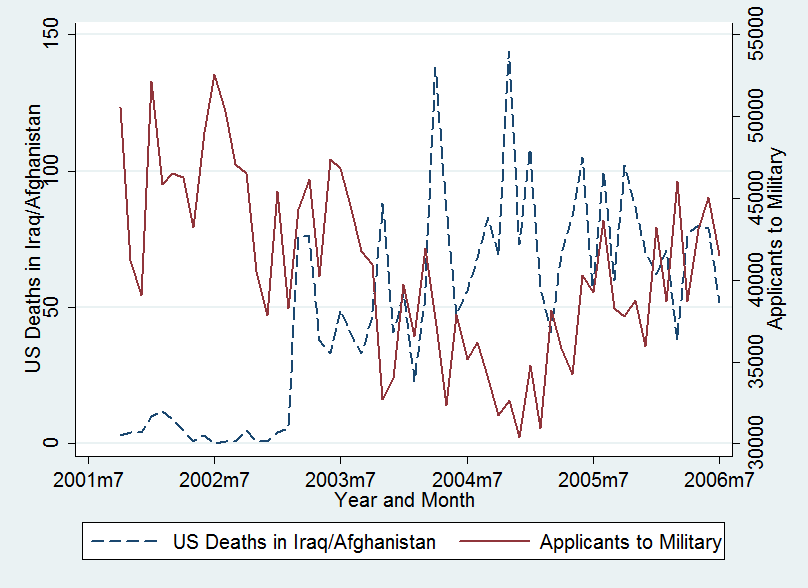
\includegraphics[scale=0.6]{../Output/graph_deathsvsrecruits_basic}
%This gets made in table1graph.do
\caption{Graph of Monthly Recruits and Monthly Iraq/Afghanistan Combat Deaths}
\label{Flo:Monthly Deaths vs. Monthly Recruits}
\end{figure} 
 
 
%Publicly available yearly figures indicate that in the period for which I have recruiting data %(1990-2006),
%the year 2000 had the lowest number of military deaths--zero from
%hostile action, but 758 from accident, illness, homicide, or suicide.
%1991 had 1787 military deaths, only 147 of which were from hostile
%action (presumably in the Persian Gulf War).


Although my analysis primarily rests on the panel nature of the data
and the inclusion of area and time fixed effects to identify the effect
of local deaths, I have also included time varying characteristics
of counties to the extent that they are available. These include unemployment
at the state and county level as reported by the Bureau of Labor Statistics, and mortality for young males age 18-24 from the Multiple Cause of Death files at the National Center for Health Statistics National Vital Statistics System. Statewide numbers of recruiters by service branch have also been included in certain specifications. 


%%%%%%%%%%%%%%%%%%%%%%%%%%%%%%%%%%%%%%%%%%%%%%%%%%%%%%%%%%%%%%%%%%%%%%%5
\section{Analysis\label{sec:Analysis}}

\subsection{Location of Origin and Rates of Death\label{sec:deathrate}}
A characteristic that affects the interpretation
of my results is the specific military occupational specialty (MOS) for which the
residents of certain counties or states are likely to sign up, and the corresponding likelihood of death faced by those in certain MOS. One could imagine that those in the infantry are more likely to be killed than those in ancillary support operations, and one could imagine that recruits from certain states are more likely than others to sign up for more dangerous occupations. However, I find that although counties do tend to send their recruits to different service branches, the rate of death faced by a recruit is statistically the same for all but a very small number of counties.  %(In the appendix, I establish the perhaps unsurprising fact that recruits and deaths are not uniformly distributed across the population. Here I restrict my attention to the likelihood of death \textit{given} enlistment.) 

The first step in this analysis is conducted with a dataset separate from the deaths and recruits data, obtained after multiple FOIA requests, showing the total enlisted employment for each of the thousands of MOS by county and month. Using the midpoint month from my analysis (March 2004), I compare each county's distribution of employment across the four service branches to the national average distribution  using Pearson's Chi-squared test. Using the observation in the dataset that I am able to match to a county, employment is split 35\% Army, 26\% Navy, 16\% Marines, and 23\% Air Force. The answer is clear that counties do not all send the same fraction of recruits to the four service branches, and thus to MOS. Without any correction for the multiplicity of hypothesis tests, as many as 1,225 of the 3,125 counties have ratios of employment that are different than that of the national average at the 95\% confidence level. Using the Bonferroni, Benjamini Hochberg, and Benjamini Krieger Yekutieli corrections indicate that 304, 901, and 977 of the 3,125 have statistically different employment distributions at the 95\% confidence level, respectively \cite{BenHoch1995, BKY2006}. Results are very similar using other months of the data.

The second step is more consequential, however. Just because counties send different fractions of their enlistees to different service branches and MOS does not mean that an enlistee from a certain county was more likely to die in Iraq or Afghanistan. To examine this issue I compare the number of recruits from a state (or county) to the number of deaths from the same state (or county). Figure \ref{Flo:HISTOstatedeaths} shows histograms of the ratio of active duty deaths to total active duty applicants for each state over the whole period for which I have data, and  Figure~\ref{Flo:HISTOcountydeaths} shows the same by county. The state ratios are centered around 0.3\%, but are clearly not all identical. I have repeated this exercise including both active duty and reserve and guard deaths (since service and death in the reserve and guard duty is clearly correlated with where one lives, including them might lead to complications) for both applicants and contracts, using both unweighted and population-weighted means. The coefficients of variation for each
of these eight methods of calculating the risk of death by state are
relatively small, ranging from 0.143 to 0.319. Looking at county figures shows that the majority of counties have zero deaths. While some counties clearly exhibit higher rates, testing is required to determine whether the variation is significant. 

%State death hazard graphs
%built by Table1graph.do
\begin{figure}
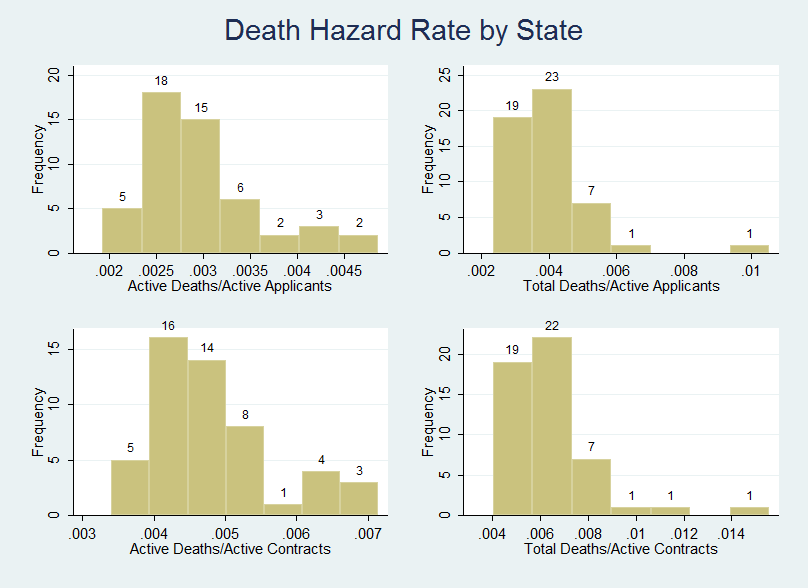
\includegraphics[scale=0.6]{../Output/hist_state_combined.png}
\caption{Death Hazard Rates by State: Active Duty/Total Deaths (2001-2010) and Active Duty Applicants/Contracts (1990-2006)}
\label{Flo:HISTOstatedeaths}
\end{figure}

%County death hazard graphs
%built by table1bycounty.do
\begin{figure}
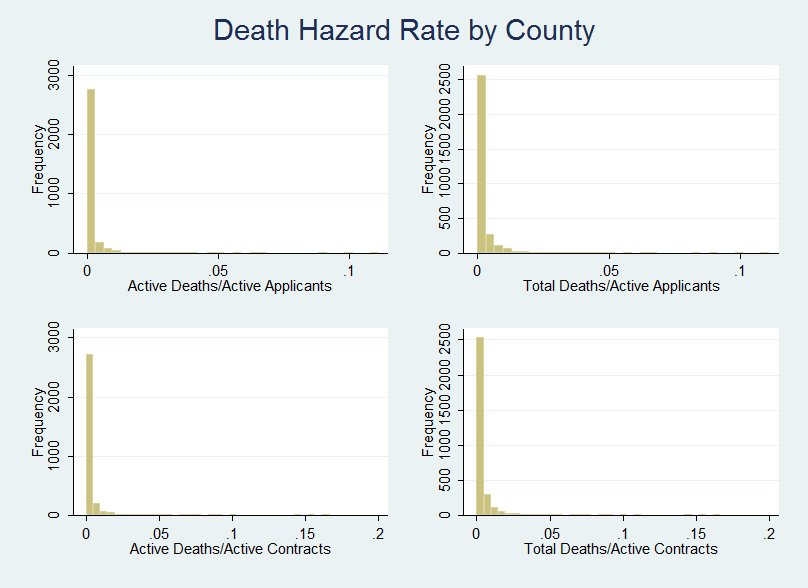
\includegraphics[scale=0.6]{../Output/hist_county_combined.png}
\caption{Death Hazard Rates by County: Active Duty/Total Deaths (2001-2010) and Active Duty Applicants/Contracts (1990-2006)}
\label{Flo:HISTOcountydeaths}
\end{figure}

To do this, I look at each individual county, and check the likelihood that it came from a binomial distribution with the hazard rate equal to that of the overall national hazard rate. (The number of active-duty deaths divided by the total number
of active duty applicants was .003.) I then tested the likelihood
that each county observation came from a binomial distribution with this
hazard rate of p=.003. Figure \ref{Flo:Pat's Histo} displays
histograms of the p-value for each state and county, one set using active-duty deaths
and active duty applicants, the other using active-duty deaths and
active-duty contracts. If counties exhibit statistically indistinguishable rates of death, then p-values should be high. The histogram displays the p-values as calculated,
but to interpret, one should, as above, use an adjustment for the high degree of multiple testing present such as Bonferroni (i.e., for states divide the cutoff for significance by the number of tests, 51, thus replacing a cutoff of .05 with 0.05/51=0.0009). Only two
of the state observations (Florida and Massachusetts) reject the null
hypothesis that their true probability is in fact .003 using applicant
data, and only one, Massachusetts, rejects using contracts data. Repeating this analysis with the 3,100 counties shows that rates of death given enlistment by county are also very rarely significantly different (eight times for applicants and zero for contracts)\footnote{The Bonferroni correction is often considered to be quite conservative. Even using much more modern methods to adjust the False Discovery Rate (FDR), I obtain similar results. Both the Benjamini Hochberg q-values and Benjamini Krieger Yekutieli sharpened q-values indicate that 16 out of the more than 3,100 counties have significantly different death rates for applicants, and zero for contracts. See \cite{BenHoch1995, BKY2006, Anderson2008} for details on estimating FDR.} So while it is the case that recruits from certain counties are more likely to enter dangerous military occupations, according to the data, the idea that the risk of death is the same across all states can only be rejected very infrequently. 

\begin{figure}
%built by Table1Graph.do AND table1bycounty.do
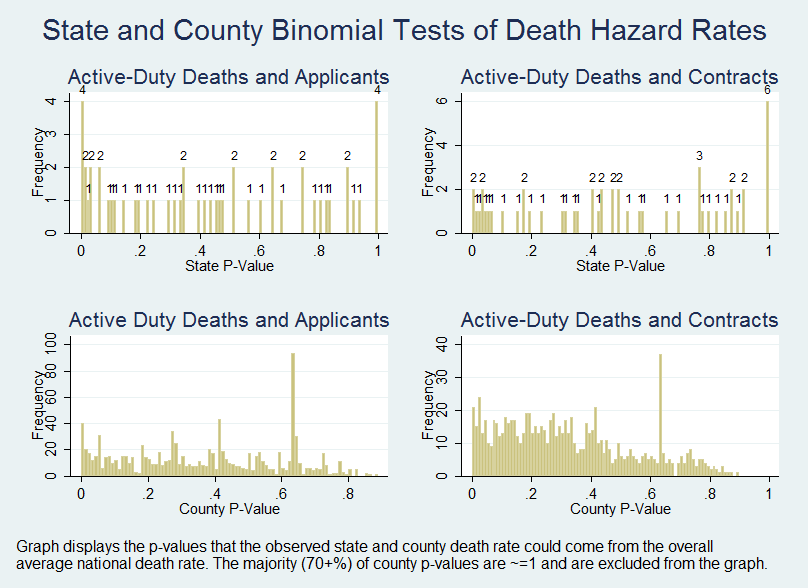
\includegraphics[scale=0.6]{../Output/hist_binomial_combined.png}
\caption{Histogram of P-Values Testing Whether Deaths Come from the
Same Binomial Distribution}
\label{Flo:Pat's Histo}
\end{figure}
\clearpage{}

This is not necessarily a reason for concern regarding omitted variable bias and my estimates of the deterrent effect of deaths,
since fixed effects for each county will still be able to control for this underlying characteristic of the state and county to the extent it is constant over time. However, it does give a slightly different meaning to the estimates I develop in the next few pages. If deaths in Iraq and Afghanistan were truly uniformly
distributed amongst all the troops, regardless of county of origin, then the fact that a soldier from a given county, say Fairfax
County, Virginia, had died would provide no more information regarding
the risk of death to a potential recruit from Fairfax County upon
enlisting than would the death of a soldier from Maricopa County,
Arizona. Any extra deterrent to enlisting because this death happened to a local soldier would thus be an emotional or behavioral response and not
an accurate updating of preferences based on risk. However, if a recruit
from Fairfax County were more likely to sign up for front-line occupations,
and those are the soldiers who were dying, then this death might actually
contain a useful signal as to the risk of death, and an extra deterrent
effect might be warranted for those reasons. Looking at the above
histograms of the rates of death by state, it seems that soldiers
from different locations have insignificantly different hazard rates, and
it is not the case that one state or another has a vastly different
rate of death of its soldiers, and the behavioral explanation is still reasonable.


%%%%%%%%%%%%%%%%%%%%%%%%%%%%%%%%%%%%%%%%%%%%%%%%%%%%%%%%%%%%%%%%%%%%%%%%
\subsection{County-Level Analysis\label{sub:County OLS}}

The primary analysis is at the county level, the smallest region at which there is close to a one-to-one relationship from death data geographic unit to recruit data geographic unit. Main results are estimated using ordinary leasts squares and a log-linear model \footnote{Log-linear estimates are calculated using Sergio Correia's reghdfe package in Stata 12 \citep{reghdfe}. Since data on recruits is in count form, the Poisson model may also be appropriate for the data, as linear models of course ignore the restriction of the dependent variable of recruits to non-negative integers. See \cite{cameron2013countdata} for a complete discussion. For the sake of robustness and transparency, I have also tested Poisson regressions, which are shown in the Appendix. The results are qualitatively very similar, showing that a death leads to slightly larger decreases in percentage terms when estimated with log-linear OLS regressions than in the Poisson regressions. The appendix also includes a negative binomial specification. Again, the results are very similar.} The regression generally follows the model:
$$Recruits_{it}=\beta_{0}Deaths_{i,t}+\beta_{1}Deaths_{i,t-1}+\beta_{2}Unemployment_{it}\\
+x'_{it}\eta+\alpha_{i}+\gamma_{t}+u_{it}$$
where Deaths implies deaths from the given county, Unemployment county unemployment, and $x$ includes in-state (but out of county) deaths as well as
state unemployment. $\alpha_{i}$ is a set of fixed effects for each county, which flexibly control for any county characteristics fixed over time such as the presence of a military base or political support for the military. $\gamma_{t}$ is a set of fixed effects for every month, so national characteristics that are the same across counties in any given time period such as the total national number of deaths, national
unemployment rate, or the military wage rate are also flexibly controlled for and cannot be separately estimated. 

% Linear with logged LHS--Main specification
% built by redefined.do
\begin{table}
\caption{}
\label{Flo:loglinear}
\scalebox{0.9}{
\documentclass[]{article}
\setlength{\pdfpagewidth}{8.5in} \setlength{\pdfpageheight}{11in}
\begin{document}
\begin{tabular}{lcccccc}
\multicolumn{7}{c}{Log County Applicants vs Deaths and Unemployment} \\ \hline
 & (1) & (2) & (3) & (4) & (5) & (6) \\
VARIABLES & Applicants & Applicants & Applicants & Contracts & Contracts & Contracts \\ \hline
 &  &  &  &  &  &  \\
Current In-County Deaths/100 & -0.352 & -0.446 & -0.569** & -0.368 & -0.443 & -0.588** \\
 & [0.381] & [0.378] & [0.279] & [0.365] & [0.355] & [0.233] \\
Lag In-County Deaths/100 & -1.031*** & -1.106*** & -1.188*** & -1.147*** & -1.184*** & -1.270*** \\
 & [0.184] & [0.195] & [0.239] & [0.233] & [0.238] & [0.284] \\
Current Out-of-County Deaths/100 &  & 0.164*** & 0.124** &  & 0.163** & 0.127* \\
 &  & [0.062] & [0.057] &  & [0.067] & [0.070] \\
Lag Out-of-County Deaths/100 &  & 0.099 & 0.049 &  & 0.017 & -0.036 \\
 &  & [0.068] & [0.058] &  & [0.084] & [0.068] \\
County Unemployment &  & 0.013** & 0.011** &  & 0.015** & 0.013** \\
 &  & [0.005] & [0.005] &  & [0.006] & [0.005] \\
State Unemployment &  & 0.005 & -0.035*** &  & 0.000 & -0.031*** \\
 &  & [0.007] & [0.008] &  & [0.007] & [0.011] \\
 &  &  &  &  &  &  \\
Observations & 178,809 & 178,739 & 178,739 & 178,809 & 178,739 & 178,739 \\
R-squared & 0.964 & 0.965 & 0.965 & 0.956 & 0.957 & 0.958 \\
County FE & YES & YES & YES & YES & YES & YES \\
Month FE & YES & YES & YES & YES & YES & YES \\
 Stateyear FE & NO & NO & YES & NO & NO & YES \\ \hline
\multicolumn{7}{c}{ Robust standard errors in brackets} \\
\multicolumn{7}{c}{ *** p$<$0.01, ** p$<$0.05, * p$<$0.1} \\
\multicolumn{7}{c}{ Notes: Table shows linear regression estimates of log (national active duty recruits +1) on deaths.} \\
\multicolumn{7}{c}{ Fixed effects are included separately by county and month, and for each state-year, as indiciated,} \\
\multicolumn{7}{c}{ The first three columns show applicants and the last three show contracts.} \\
\multicolumn{7}{c}{ Filename:LNLinearW.tex} \\
\end{tabular}
\end{document}

}
\end{table}


Table \ref{Flo:loglinear}
shows the results when linear regression is used to analyze the data
at the county-month level. The left half of these regressions show the analysis done for applicants, the right hand side for contracts, one step further in the recruiting
process. %The first specification, for applicants in column one and contracts in column five, is the `horse race' specification, comparing in-county deaths, out-of-county but in-state deaths,  and out-of-state deaths. Of course this precludes the inclusion of monthly fixed effects, so this model is mis-specified to the extent that there is temporal heterogeneity in the recruiting response to deaths over the course of the wars, nevertheless, I find it illustrative that the coefficient for lagged in-county deaths is nearly five times that of the coefficient for an out-of-state death (1\% compared to 0.2\%). (A more detailed analysis of deaths at the national level is presented in the appendix.)
Fixed effects for each county and for each month are included in all specifications, as well as state-year fixed effects  in specifications 3 and 6.
Observations are weighted by county population, and standard errors
are clustered by county. The results indicate that one additional
in-county death is followed in the next month by a 1.1\%
decrease in applicants and a similar reduction in contracts.
\footnote{Note that all death figures have been divided by 100 to make more
useful digits of the coefficients visible, and thus all coefficients
for deaths should be interpreted as percents and not fractions (i.e.
0.4 is 0.4 percent, not 40 percent).} Deaths from in-state but out-of-county
appear to have a small positive effect, from 0.1\% to 0.2\%, which leads to some concern about the possible behavioral interpretation of my results---perhaps recruiters avoid an area after a death and instead spend their time recruiting from neighboring areas. This alternative mechanism, however, is complicated by estimates below showing that deaths in contiguous counties do not lead to an increase in recruiting. 

Unemployment at the state level has a negative effect: a one percentage point increase leads to a small but not always significant decrease in recruiting,
while a one percentage point increase in county unemployment leads
to a 1\% increase in recruiting.\footnote{It should not be surprising that specifications including both county and state unemployment show one positive and one negative coefficient: holding state unemployment constant and increasing county unemployment means the county in question is relatively unlucky within the state, so recruits in that county have fewer other options and are more likely to enlist. Conversely, hold county unemployment constant and increase state unemployment, and the county is relatively lucky employment-wise, leading to fewer recruits.}  A simple comparison of the coefficients on lagged county deaths and county unemployment indicates that one fewer death of a soldier from the county would lead to the same increase in recruiting as a one percentage point increase in county unemployment.

%Unemployment levels are also closely correlated with recruiting levels.
%State unemployment has fairly volatile estimates depending on which
%fixed effects are included, but coefficients for county unemployment
%are stable; a one percentage point increase in county unemployment
%leads to two to four more recruits.

%One could conceivably be concerned that county unemployment was measured
%somewhat inaccurately and in a way that somehow biased the estimates,
%especially given the relatively small sample size used to calculate
%each county's unemployment rate and its mechanical relationship to
%state and national unemployment levels. I have tested this by adding
%normally distributed noise to the county unemployment estimates; none
%of the other estimates changed significantly.

The idea that potential recruits are responding to county and state
unemployment above and beyond the national unemployment level is in
accordance with rational utility-maximizing individuals, assuming
that moving across county or state lines (or finding employment across
county or state lines) is costly, as county and state unemployment
levels directly affect one's likelihood of employment, and thus income
and utility. As shown in section~\ref{sec:deathrate}, deaths of active duty soldiers from one's own county
or state are unrelated to one's own likelihood of dying in the service,
since the Army operates at a national level and recruits are put into
military careers irrespective of their state or county of origin (at
least to the extent discussed above). Clearly this is not quite the
case with Reserve and National Guard troops, as Reservists simply
report to the nearest base for one weekend a month and two weeks
a year of training, but their recruiting numbers are not included
in this analysis.


This analysis has been done using all of active duty, reserve, and
guard duty deaths. I do this because the main emphasis of my analysis
is to determine the magnitude of the observed reaction to deaths.
It may be true that the response to deaths of local soldiers from
reserve and guards units is a rational response based on an updated
assessment of the risk of death (since those who enlist would serve in the same location-based reserve or guard unit) but still, the magnitude of the observed
deterrence effect, rational or not, would be what is of interest to
policy makers. As a robustness check, however, I have run the analysis
using only the active-duty deaths, and under this specification, in-county
deaths are followed by a similar or slightly larger reduction in recruits in the
next month. The coefficients for out-of-county deaths and unemployment also
remain similar. These results are shown in Appendix Table~\ref{Flo:Rdeathslinear}. 

%%%%%%%%%%%%%%%%%%%%%%%%%%%%%%%%%%%%%%%%%%%%%%%%%%%%%%%
\paragraph{Additional Controls}

Despite the inclusion of fixed effects, the potential for omitted
variable bias still exists. One of the most obvious ways this might
occur is through the action of the military's production recruiters.
It seems likely that the number of production recruiters is positively
correlated with the number of recruits, and in the extreme this is
clearly true mechanically. If the number of recruiters (or their level
of effort) were also correlated with the number of deaths, my estimates
would be biased. Given that recruiters serve for three years in one
place, it is highly unlikely that the military is relocating them
in a way that is correlated with monthly deaths. Without being relocated,
however, recruiters may change their level of effort. FOIA requests for data on recruiter quotas unfortunately have not been granted, so I am only able to use the number of recruiters by state and quarter until halfway through 2004\footnote{I am grateful to John Warner for sharing this data.}, which I have included as an extra control variable for that portion of the sample. I also have detailed mortality data through 2004. It is conceivable that deaths unrelated to
the military would play a role in determining recruiting (for example,
young men in a crime-ridden community may be anxious to join the military
as a means of escape) thus I include monthly male 18-24 year-old mortality figures
as well. Table \ref{Flo:LNRec&Mort} shows these results. The
analysis is done for both applicants and contracts, with the observations
limited to October 2001 to June 2004. County and monthly
fixed effects are included. The estimates are similar in this restricted time period to those from the full sample, and the effect of a death does not change significantly when I add the extra controls. (Comparing column 1 to 2 and 3 to 4.)  %The estimates for contracts are only
%about half of what they are using the full data set, indicating that
%the response to deaths is not constant over the duration of the entire sample.

\begin{table}
%built by interactionscontrols.do
\caption{Recruiter and Mortality Controls}
\label{Flo:LNRec&Mort}\documentclass[]{article}
\setlength{\pdfpagewidth}{8.5in} \setlength{\pdfpageheight}{11in}
\begin{document}
\begin{tabular}{lcccc} \hline
 & (1) & (2) & (3) & (4) \\
VARIABLES & Applicants & Applicants & Contracts & Contracts \\ \hline
 &  &  &  &  \\
Current In-County Deaths/100 & -0.740** & -0.634** & -0.406 & -0.356 \\
 & [0.298] & [0.305] & [0.327] & [0.318] \\
Lag In-County Deaths/100 & -1.096** & -1.077*** & -0.732* & -0.731* \\
 & [0.443] & [0.391] & [0.406] & [0.383] \\
Current Out-of-County Deaths/100 & 0.216** & 0.293*** & 0.195** & 0.239*** \\
 & [0.093] & [0.094] & [0.095] & [0.089] \\
Lag Out-of-County Deaths/100 & 0.230** & 0.310*** & 0.083 & 0.141 \\
 & [0.101] & [0.102] & [0.100] & [0.099] \\
State Unemployment & -0.010 & -0.009 & -0.008 & -0.008 \\
 & [0.009] & [0.009] & [0.009] & [0.009] \\
County Unemployment & 0.019*** & 0.019*** & 0.017*** & 0.017*** \\
 & [0.002] & [0.002] & [0.002] & [0.002] \\
Military Recruiter by State &  & 0.023** &  & 0.020* \\
 &  & [0.010] &  & [0.011] \\
Lag County Mortality Rate &  & 0.001* &  & 0.000 \\
 &  & [0.000] &  & [0.000] \\
Lag Out-of-County Mortality Rate &  & 0.000 &  & -0.000 \\
 &  & [0.000] &  & [0.000] \\
 &  &  &  &  \\
Observations & 97,794 & 97,794 & 97,794 & 97,794 \\
R-squared & 0.968 & 0.968 & 0.962 & 0.962 \\
County FE & YES & YES & YES & YES \\
Month FE & YES & YES & YES & YES \\
 Stateyear FE & NO & NO & NO & NO \\ \hline
\multicolumn{5}{c}{ Robust standard errors in brackets} \\
\multicolumn{5}{c}{ *** p$<$0.01, ** p$<$0.05, * p$<$0.1} \\
\multicolumn{5}{c}{ Notes: Table shows linear regression estimates of log (national active duty recruits +1) on deaths.} \\
\multicolumn{5}{c}{ Fixed effects are included separately by county and month, and for each state-year, as indiciated,} \\
\multicolumn{5}{c}{ The first four columns show applicants and the last three show contracts.} \\
\multicolumn{5}{c}{ Filename:LNcontrolW.tex} \\
\end{tabular}
\end{document}

\end{table}

Another interesting test of these results is shown in Table \ref{Flo:Media}.
Here I have included the number of deaths that occurred in contiguous
counties and the number of deaths that occurred in counties that share
the same media market as the main county of interest. County contiguity
is defined using the 1991 ICPSR contiguous county file.\footnote{U.S. Dept. of Commerce, Bureau of the Census. CONTIGUOUS COUNTY FILE,
1991: {[}UNITED STATES{]} {[}Computer file{]}. Washington, DC: U.S.
Dept. of Commerce, Bureau of the Census {[}producer{]}, 1992. Ann
Arbor, MI: Inter- university Consortium for Political and Social Research
{[}distributor{]}, 1992. doi:10.3886/ICPSR09835 
} Media markets are defined using the Nielsen Media Research's Designated
Market Area (DMA). In the year 2000, Nielsen divided the country into 208 DMAs based on a preponderence of residents having access to the same broadcast television and radio stations.   (See \cite{DMAsource1} and \cite{DMAsource2} for more details.) The regressions show that deaths in nearby areas, whether defined using county borders or media market, have smaller effects on recruiting in a given county. The effect size is roughly half as large as that of a death from the county. While it seems that recruits do respond to information from outside the county, this is perhaps suggestive evidence that the county response to deaths is due to something more than information, since media markets are intended to share major news sources. 

%MEDIA MARKET AND CONTIGUOUS
\begin{table}
%built by redefcontig.do
\caption{Deaths in Neighboring Counties and Same Media Market}
\label{Flo:Media}
\scalebox{0.65}{\documentclass[]{article}
\setlength{\pdfpagewidth}{8.5in} \setlength{\pdfpageheight}{11in}
\begin{document}
\begin{tabular}{lcccccccccc}
\multicolumn{11}{c}{Media and Contiguous Deaths} \\ \hline
 & (1) & (2) & (3) & (4) & (5) & (6) & (7) & (8) & (9) & (10) \\
VARIABLES & Applicants & Applicants & Applicants & Applicants & Applicants & Contracts & Contracts & Contracts & Contracts & Contracts \\ \hline
 &  &  &  &  &  &  &  &  &  &  \\
Current In-County Deaths/100 &  & -0.541* &  & -0.533* & -0.540* &  & -0.514** &  & -0.509** & -0.528** \\
 &  & [0.291] &  & [0.282] & [0.284] &  & [0.237] &  & [0.232] & [0.234] \\
Lag In-County Deaths/100 &  & -1.005*** &  & -1.123*** & -1.134*** &  & -1.015*** &  & -1.183*** & -1.183*** \\
 &  & [0.250] &  & [0.258] & [0.256] &  & [0.280] &  & [0.314] & [0.313] \\
Death in Neighbor County & -0.222 & -0.141 &  &  &  & -0.431** & -0.353 &  &  &  \\
 & [0.144] & [0.163] &  &  &  & [0.200] & [0.222] &  &  &  \\
Lag Death in Neighbor County & -0.587*** & -0.505** &  &  &  & -0.720*** & -0.636*** &  &  &  \\
 & [0.212] & [0.212] &  &  &  & [0.227] & [0.223] &  &  &  \\
State Unemployment & -0.036*** & -0.037*** & 0.004 & -0.036*** & -0.035*** & -0.032*** & -0.033*** & -0.001 & -0.032*** & -0.031*** \\
 & [0.008] & [0.008] & [0.011] & [0.008] & [0.008] & [0.011] & [0.011] & [0.011] & [0.011] & [0.011] \\
County Unemployment & 0.011** & 0.011** & 0.012** & 0.011** & 0.011** & 0.013** & 0.013** & 0.014** & 0.013** & 0.013** \\
 & [0.005] & [0.005] & [0.006] & [0.005] & [0.005] & [0.005] & [0.005] & [0.006] & [0.005] & [0.005] \\
Death in Media Market &  &  & -0.399 & -0.078 & -0.171 &  &  & -0.800** & -0.355* & -0.485** \\
 &  &  & [0.267] & [0.159] & [0.172] &  &  & [0.364] & [0.193] & [0.201] \\
Lag Death in Media Market &  &  & -0.802*** & -0.457** & -0.537*** &  &  & -1.150*** & -0.692*** & -0.728*** \\
 &  &  & [0.298] & [0.193] & [0.205] &  &  & [0.352] & [0.220] & [0.236] \\
Current Out-of-County Deaths/100 &  &  &  &  & 0.145** &  &  &  &  & 0.193** \\
 &  &  &  &  & [0.063] &  &  &  &  & [0.075] \\
Lag Out-of-County Deaths/100 &  &  &  &  & 0.128** &  &  &  &  & 0.069 \\
 &  &  &  &  & [0.065] &  &  &  &  & [0.080] \\
 &  &  &  &  &  &  &  &  &  &  \\
Observations & 178,568 & 178,568 & 178,739 & 178,739 & 178,739 & 178,568 & 178,568 & 178,739 & 178,739 & 178,739 \\
R-squared & 0.965 & 0.965 & 0.965 & 0.965 & 0.965 & 0.958 & 0.958 & 0.957 & 0.958 & 0.958 \\
County FE & YES & YES & YES & YES & YES & YES & YES & YES & YES & YES \\
Month FE & YES & YES & YES & YES & YES & YES & YES & YES & YES & YES \\
 Stateyear FE & NO & NO & NO & NO & NO & NO & NO & NO & NO & NO \\ \hline
\multicolumn{11}{c}{ Robust standard errors in brackets} \\
\multicolumn{11}{c}{ *** p$<$0.01, ** p$<$0.05, * p$<$0.1} \\
\multicolumn{11}{c}{ Notes: Table shows linear regression estimates of log (national active duty recruits +1) on deaths.} \\
\multicolumn{11}{c}{ Fixed effects are included separately by county and month as indiciated,} \\
\multicolumn{11}{c}{ The first five columns show applicants and the last five show contracts.} \\
\multicolumn{11}{c}{ Filename:redefcontigLN.tex} \\
\end{tabular}
\end{document}

}
\end{table}

\subsection{Lags and Leads of Deaths and Unemployment\label{sub:Lags}}
My main empirical method thus far has been to compare county recruits
in a given calendar month to county-wide and state-wide deaths in
the previous month. It is possible that potential recruits initially
deterred from enlisting by a death eventually {}``forget'' about
local deaths and join the military. Table~\ref{Flo:Cumulative LagsLN}
shows regressions with cumulative death and unemployment lags
of two, four, six, and twelve months--that is, the sum of current
deaths plus all the deaths that occurred in the previous number of
months. The results indicate that deaths from previous months have a significantly smaller deterrent effect on recruiting than more recent deaths. Earlier regressions have shown a deterrent effect of over one percent for deaths in the previous month; these
regressions show a relative decline in the effect size the longer a time period included. The effect size decreases to one third a percent for applicants for twelve months of lagged deaths. The decline in effect size does not appear to be as steady for contracts. Poisson regressions produce very similar semi-elasticity
estimates.

%Cumulative Lags
\begin{table}
%builtby redefrunninglags.do
\caption{Cumulative Lags}
\label{Flo:Cumulative LagsLN}
\scalebox{0.75}{\documentclass[]{article}
\setlength{\pdfpagewidth}{8.5in} \setlength{\pdfpageheight}{11in}
\begin{document}
\begin{tabular}{lcccccccc} \hline
 & (1) & (2) & (3) & (4) & (5) & (6) & (7) & (8) \\
VARIABLES & Applicants & Applicants & Applicants & Applicants & Contracts & Contracts & Contracts & Contracts \\ \hline
 &  &  &  &  &  &  &  &  \\
Cum. 2 Lags Out-of-County Deaths & 0.087** &  &  &  & 0.052 &  &  &  \\
 & [0.042] &  &  &  & [0.049] &  &  &  \\
Cum. 2 Lags In-County Deaths & -0.775*** &  &  &  & -0.685*** &  &  &  \\
 & [0.186] &  &  &  & [0.218] &  &  &  \\
Cum. 2 Lags State Unemployment & 0.323 &  &  &  & 0.178 &  &  &  \\
 & [0.226] &  &  &  & [0.256] &  &  &  \\
Cum. 2 Lags County Unemployment & 0.321* &  &  &  & 0.431** &  &  &  \\
 & [0.194] &  &  &  & [0.215] &  &  &  \\
Cum. 4 Lags  Out-of-County Deaths &  & 0.061 &  &  &  & 0.046 &  &  \\
 &  & [0.037] &  &  &  & [0.044] &  &  \\
Cum. 4 Lags  In-County Deaths &  & -0.627*** &  &  &  & -0.629*** &  &  \\
 &  & [0.148] &  &  &  & [0.193] &  &  \\
Cum. 4 Lags  State Unemployment &  & 0.465** &  &  &  & 0.229 &  &  \\
 &  & [0.187] &  &  &  & [0.211] &  &  \\
Cum. 4 Lags  County Unemployment &  & 0.060 &  &  &  & 0.234 &  &  \\
 &  & [0.170] &  &  &  & [0.192] &  &  \\
Cum. 6 Lags  Out-of-County Deaths &  &  & 0.063** &  &  &  & 0.062* &  \\
 &  &  & [0.031] &  &  &  & [0.036] &  \\
Cum. 6 Lags  In-County Deaths &  &  & -0.539*** &  &  &  & -0.667*** &  \\
 &  &  & [0.111] &  &  &  & [0.140] &  \\
Cum. 6 Lags  State Unemployment &  &  & 0.467*** &  &  &  & 0.218 &  \\
 &  &  & [0.137] &  &  &  & [0.157] &  \\
Cum. 6 Lags  County Unemployment &  &  & -0.032 &  &  &  & 0.116 &  \\
 &  &  & [0.133] &  &  &  & [0.153] &  \\
Cum. 12 Lags Out-of-County Deaths &  &  &  & 0.041* &  &  &  & 0.060** \\
 &  &  &  & [0.024] &  &  &  & [0.026] \\
Cum. 12 Lags In-County Deaths &  &  &  & -0.354*** &  &  &  & -0.589*** \\
 &  &  &  & [0.096] &  &  &  & [0.107] \\
Cum. 12 Lags State Unemployment &  &  &  & 0.090 &  &  &  & -0.035 \\
 &  &  &  & [0.093] &  &  &  & [0.108] \\
Cum. 12 Lags County Unemployment &  &  &  & 0.167* &  &  &  & 0.227* \\
 &  &  &  & [0.098] &  &  &  & [0.118] \\
 &  &  &  &  &  &  &  &  \\
Observations & 175,595 & 169,321 & 163,047 & 144,225 & 175,595 & 169,321 & 163,047 & 144,225 \\
R-squared & 0.965 & 0.965 & 0.965 & 0.964 & 0.957 & 0.957 & 0.957 & 0.957 \\
County FE & YES & YES & YES & YES & YES & YES & YES & YES \\
Month FE & YES & YES & YES & YES & YES & YES & YES & YES \\
 Stateyear FE & NO & NO & NO & NO & NO & NO & NO & NO \\ \hline
\multicolumn{9}{c}{ Robust standard errors in brackets} \\
\multicolumn{9}{c}{ *** p$<$0.01, ** p$<$0.05, * p$<$0.1} \\
\multicolumn{9}{c}{ Notes: Table shows linear regression estimates of log (national active duty recruits +1) on cumulative} \\
\multicolumn{9}{c}{ lagged deaths. Fixed effects are included separately by county and month as indiciated,} \\
\multicolumn{9}{c}{ The first five columns show applicants and the last five show contracts.} \\
\multicolumn{9}{c}{ Filename:runninglagsLN.tex} \\
\end{tabular}
\end{document}
}
\end{table}

As a robustness check on my main specification, I have also run regressions including deaths one month into the future. In the main log-linear specification, deaths from the same county one month into the future appear to have small but statistically significant relationships with recruits. However, the Poisson models, as well as the log-linear model using only active duty deaths, show clearly that deaths in the future do not correlate signficantly with current recruiting levels.  These regressions are shown in Appendix Table~\ref{Flo:forwardbasicLN} and Table~\ref{Flo:forwardPbasic}. 

\subsection{Heterogeneity of the Deterrent Effect\label{sub:interactions}}

The analysis in the previous two subsections makes it clear that in-county
deaths result in a significant decrease in county recruiting. An important
corollary question concerns the heterogeneity of this effect.
All counties are unlikely to observe the same deterrent effect of
death. Here I investigate the recruiting response to deaths based
on a county's demographic and cultural makeup, specifically, its population,
unemployment, racial makeup, rural/urban status, and political alignment.
Table \ref{Flo:Linear Interactions} displays these regressions.
They all include monthly and county fixed effects, out of county but
in-state deaths, as well as unemployment, and I have added county
characteristics interacted with lagged in-county deaths. All variables
to be interacted have had the population weighted mean subtracted. %\footnote{ In a standard OLS regression this de-meaning would mean we could expect the main coefficient on lagged county deaths to remain essentially constant, but the weighting scheme used in Poisson regressions does not give the same sort of results. I have tested this and found that the main coefficient does stay very stable in least squares regressions regardless of what sort of weighted de-meaned interaction variables are included. I have also run these regressions using least squares and the results are qualitatively similar.}
Note that most of the county characteristics are fixed over time and thus perfectly collinear with fixed effects and cannot also be included.

%LINEAR INTERACTIONS
%built by interactionscontrols.do
\begin{table}
\caption{Linear Interactions}
\label{Flo:Linear Interactions}\documentclass[]{article}
\setlength{\pdfpagewidth}{8.5in} \setlength{\pdfpageheight}{11in}
\begin{document}
\begin{tabular}{lc} \hline
 & (1) \\
VARIABLES & Applicants \\ \hline
 &  \\
Current In-County Deaths/100 & -0.501 \\
 & [0.381] \\
Lag In-County Deaths/100 & -0.686 \\
 & [0.480] \\
Current Out-of-County Deaths/100 & 0.165*** \\
 & [0.061] \\
Lag Out-of-County Deaths/100 & 0.083 \\
 & [0.069] \\
Lag County Death*County Unemployment & 0.007 \\
 & [0.004] \\
Lag County Death/County Population & 2.698 \\
 & [1.984] \\
Lag County Death*\%Black Population & -0.065** \\
 & [0.033] \\
Lag County Death*\%George Bush Vote & 0.092*** \\
 & [0.030] \\
Lag County Death*Rural & -0.029 \\
 & [0.034] \\
State Unemployment & 0.005 \\
 & [0.007] \\
County Unemployment & 0.012** \\
 & [0.006] \\
 &  \\
Observations & 177,371 \\
R-squared & 0.965 \\
County FE & YES \\
Month FE & YES \\
 Stateyear FE & NO \\ \hline
\multicolumn{2}{c}{ Robust standard errors in brackets} \\
\multicolumn{2}{c}{ *** p$<$0.01, ** p$<$0.05, * p$<$0.1} \\
\multicolumn{2}{c}{ Notes: Table shows linear regression estimates of log (national active duty recruits +1) on deaths.} \\
\multicolumn{2}{c}{ Fixed effects are included separately by county and month, and for each state-year, as indiciated,} \\
\multicolumn{2}{c}{ The first three columns show applicants and the last three show contracts.} \\
\multicolumn{2}{c}{ Filename:LNinteractCOMBINE.tex} \\
\end{tabular}
\end{document}

\end{table}

I have interacted lagged county deaths with inverse county population to estimate the effect in terms of deaths per population. Also included are interactions with the monthly county unemployment figure (the only county characteristic
that changes over time and thus is not collinear with the fixed effects
and can be included in the regression by itself), percent African-American
population as measured in 2005, %racial fractionalization using percent white, black, Native American, Asian, and Pacific Islander, 
a binary measure of rural status using the USDA's Economic Research Service classification, and the percent of the county that voted for George Bush in 2004.
The regressions are run for applicants and contracts.%, the first column with percent black, and the second with racial fractionalization.
I have also run regressions including interactions of all these same
variables, but interacted with all four counts of deaths (in and out
of county, lagged and current) the coefficients on the original interaction
are very similar, and the coefficients for the interactions with out-of-county
deaths and current in-county deaths all either go in the same direction
as the ones shown in Table \ref{Flo:Linear Interactions} or are
statistically not different than zero. 


%Deaths per Male 18-24 year-old County Population has a rather large and negative coefficient, which is actually quite reasonable. The coefficient implies that there is a level effect of deaths, and then an additional effect of deaths per capita, from -2086 to -2215 for applicants and a statistically insignificant -1510 to -1704 for contracts. This means that an increase of one death for every one young male (obviously improbably high) would result in a decrease of recruits by 1500 to 2000 percent (also improbably high). Simpler to imagine is that for every additional 1500 to 2000 young males in a county, the deterrent effect of deaths is one percent less negative. More-populated counties have a smaller percentage recruiting response to deaths than less-populated counties. With more people, perhaps other young men are less likely to hear the news of the death of a soldier, and if they hear it, perhaps they are less likely to have known the soldier who was killed and thus be relatively undeterred by his death. It is slightly puzzling, however, why this differential effect would be so strongly significant for applicants and not significant for contracts. 

Death {*} County Unemployment yields positive but insignificant estimates
for applicants and small but significant estimates for contracts,
indicating that deaths in counties with higher unemployment are not
as large a deterrent effect, and could potentially even make the recruiting response
to deaths positive. %Under the first specification for contracts, a county with the weighted average level of county unemployment (5.5\% in the sample) would have a 0.5\% reduction in recruits for every death. A county with 6.5\% unemployment would actually see a 0.5+ (6.5-5.5)*0.8=1.3\% increase in recruiting with every death (not to mention the 1.6\% increase in recruiting thanks to the level effect of county unemployment) . 

The percentage of county population that is African-American increases
the size of the effect of a death. A county with the weighted average
proportion of the population (13\%) African-American would see a 0.7\%
reduction in applicants for every death, a county with one standard deviation
(13\%) higher African-American population would see a -0.7+(13\%{*}-0.065)=1.55\%
reduction in recruits for each death. The estimates are slightly large for contracts than for applicants. %I have also done the analysis using racial fractionalization, a more detailed description of the racial makeup of counties instead of simply percent African-American, but these estimates are not significant.

Rural is a binary measure of whether the county is rural using USDA's Rural-Urban continuum, which is partly a measure of population and partly distance from a metropolitan area. The estimate is insignificant, but the sign does seem to go in the same direction as population, however, indicating that rural counties
(with lower populations not neighboring metropolitan areas) would have larger negative recruiting responses to deaths. Deaths per Male 18-24 year-old County Population has a positive but only marginally significant coefficient. This indicates that perhaps the size of the county does not strongly affect how its population responds to a death. %Running the regressions without the rural interaction does not change the coefficient on the population interaction significantly.

Finally, I have interacted the county percent of the vote that went
to George Bush in 2004 with deaths. The coefficient estimates are 0.09\% for applicants to 0.15\% for contracts. This indicates that a county with the weighted mean Bush voteshare would see a decrease in applicants of 0.7\% for every death, but a county with one percentage point higher vote for Bush would see a 0.09\% smaller (closer
to zero) decrease in recruiting. This indicates that a county with
roughly 6 to 8 percentage point higher than the weighted average Bush
vote would see \textit{increases} in recruiting after deaths. The average Bush
vote share is 50.6\%, and the standard deviation is nearly 14 percentage
points. Well over half the counties had a Bush vote share over 57\%, which indicates that the prospect of an increase in recruiting due to deaths is not at all unlikely.

As shown in \cite{Ted-Miguel-Bush-Deaths}, at least at the state
level, war deaths led to poorer Bush election performance in 2004.
As a robustness check I have replaced the Bush '04 vote share with
Bush '00 county vote-share, which was obviously unaffected by Iraq
and Afghanistan combat deaths. The estimates are nearly identical. 

These estimates all show that county characteristics are very important
in determining the response of a county's potential recruits to the
news of a death. High unemployment may dampen the deterrent effect of deaths slightly.
Counties with higher fractions of African-American population have
a larger response to deaths, as did counties that voted against George
W. Bush (in either 2000 or 2004).


%%%%%%%%%%%%%%%%%%%%%%%%%%%%%%%%%%%%%%%%%%%%%%%%%%%%%%%%%%%%
\subsection{Recruiting Response for Different Types of Recruits \label{sub:Different Recruit Types}}


The military, like any other organization, has a strong interest in
recruiting high quality employees. The services have generally held {}``high
quality'' to mean a person in possession of a high school degree
and a score of 50 or higher on the AFQT. The services have often had
separate quotas for high and low quality enlistees, and they have
generally required that a high percentage of their recruits fall into
the high category, although these requirements have changed over time
with the needs of the services. 

%LN QUALITY OF RECRUIT
\begin{table}
\caption{Recruits by Quality}
\label{Flo: Recs by QualityLN}
\scalebox{0.75}{\rotatebox{90}{
{\documentclass[]{article}
\setlength{\pdfpagewidth}{8.5in} \setlength{\pdfpageheight}{11in}
\begin{document}
\begin{tabular}{lcccccccc} \hline
 & (1) & (2) & (3) & (4) & (5) & (6) & (7) & (8) \\
VARIABLES & LQ Applicants & HQ50 Applicants & HQ50-Alt. Applicants & HQ75 Applicants & LQ Contracts & HQ50 Contracts & HQ50-Alt. Contracts & HQ75 Contracts \\ \hline
 &  &  &  &  &  &  &  &  \\
In-County Deaths/100 & -0.439 & -0.828* & -0.463 & -1.123 & -0.802** & -0.468 & -0.269 & 0.870 \\
 & [0.364] & [0.444] & [0.438] & [0.868] & [0.362] & [0.340] & [0.355] & [1.207] \\
Lag In-County Deaths/100 & -1.249*** & -1.309*** & -1.217*** & -3.687*** & -1.549*** & -1.113*** & -1.371*** & -4.115*** \\
 & [0.242] & [0.391] & [0.285] & [0.481] & [0.327] & [0.288] & [0.272] & [1.151] \\
Out-of-County Deaths/100 & 0.175** & 0.114 & 0.204*** & 0.093 & 0.148* & 0.092 & 0.139* & -0.029 \\
 & [0.076] & [0.087] & [0.069] & [0.204] & [0.083] & [0.087] & [0.079] & [0.187] \\
Lag Out-of-County Deaths/100 & 0.025 & 0.111 & 0.193** & 0.015 & -0.077 & 0.035 & 0.052 & -0.063 \\
 & [0.079] & [0.088] & [0.080] & [0.194] & [0.103] & [0.100] & [0.094] & [0.241] \\
State Unemployment & -0.002 & 0.024*** & 0.022*** & 0.031*** & -0.011 & 0.021** & 0.018** & 0.027*** \\
 & [0.007] & [0.008] & [0.007] & [0.010] & [0.008] & [0.008] & [0.008] & [0.011] \\
County Unemployment & 0.011** & 0.017*** & 0.011* & 0.004 & 0.012** & 0.019*** & 0.014** & 0.010** \\
 & [0.005] & [0.006] & [0.006] & [0.004] & [0.006] & [0.006] & [0.006] & [0.004] \\
 &  &  &  &  &  &  &  &  \\
Observations & 178,739 & 178,739 & 178,739 & 178,739 & 178,739 & 178,739 & 178,739 & 178,739 \\
R-squared & 0.952 & 0.940 & 0.951 & 0.788 & 0.937 & 0.930 & 0.943 & 0.720 \\
County FE & YES & YES & YES & YES & YES & YES & YES & YES \\
Month FE & YES & YES & YES & YES & YES & YES & YES & YES \\
 Stateyear FE & NO & NO & NO & NO & NO & NO & NO & NO \\ \hline
\multicolumn{9}{c}{ Robust standard errors in brackets} \\
\multicolumn{9}{c}{ *** p$<$0.01, ** p$<$0.05, * p$<$0.1} \\
\multicolumn{9}{c}{ Notes: Table shows linear regression estimates of log (national active duty recruits +1) on cumulative} \\
\multicolumn{9}{c}{ lagged deaths. Fixed effects are included separately by county and month as indiciated,} \\
\multicolumn{9}{c}{ The first four columns show applicants and the last four show contracts.} \\
\multicolumn{9}{c}{ Filename:highqualitybytypeLN.tex} \\
\end{tabular}
\end{document}
}}}
\end{table}

Table \ref{Flo: Recs by QualityLN} shows results for recruits
of different quality levels. I have broken recruits into four groups, the first three of which attempt to use definitions explicitly used by the military.
Low Quality recruits either scored below 50 on the AFQT or do not
have a high school degree. High Quality have both a 50 or higher on
the AFQT as well as a high school degree. High Quality-Alt scored
50 or higher on the AFQT but may still be in their senior year of
high school (many recruits sign contracts while they are still in
school, but join through the Delayed Entry Program, so they do not
actually ship out until they graduate and are considered high quality
recruits by the military.) Very High Quality recruits is not a specific
distinction used by the military, but is meant to identify the most
sought after recruits--those who have a 75 or higher on the AFQT and
have taken at least some college courses. %There are fewer observations in this specification since 666 counties never have a very high quality recruit and cannot be included. 
The results indicate that all but the Very High Quality recruits have roughly the same response to deaths: a 1\% reduction in recruits for every
death. Amongst Very High Quality recruits, the effect is almost 4\%.%
\footnote{It may be slightly surprising that higher-quality recruits are more
deterred by local deaths if one interprets the response to a county
death as an {}``over-response'' compared to deaths from out of county
or out of state, since higher quality recruits are better-educated
and might be expected to read national newspapers or acquire information
about distant deaths with lower cost. Indeed regressions not shown
indicate that the response to out-of-county and out-of-state deaths
is no larger for higher quality recruits than for lower quality recruits.
However, the results are consistent with a story of the local-death-deterrent
being due to personal knowledge of the soldier who was killed, since
evidence indicates that those with more education are likely to have
larger social networks. As written in \cite{GlaeserSocialNetworks},
{}``The connection between social capital and human capital is one
of the most robust empirical regularities in the social capital literature.''} 

%Another interesting difference is the effect of unemployment on different types of recruits. \emph{A priori} it is unclear how unemployment would affect different types of recruits. Higher unemployment could raise low quality enlistment because low quality individuals have fewer outside options, or it could hurt low quality individuals, because high quality individuals have their outside options eliminated, then they join the military in greater numbers, and there isn't enough demand remaining for low quality individuals to enlist. (While High Quality can typically enlist in the military at any time with no cap on demand, low quality recruiting is frequently subject to both demand and supply constraints.) The table seems to indicate that county unemployment leads to a 2.5\% increase in high quality recruiting and a 1.5\% increase in low quality recruits. 
Again, I have tested whether the results are the same when done using Poisson regression, and the results exhibit the same patterns for deaths---very high quality recruits are more deterred by deaths than other types of recruits.

%The appendix includes a similar analysis in Table \ref{Flo:Recruits by Service} with recruits broken out by military service branch.

\subsection{Recruiting Response for Different Types of Deaths\label{sub:Different Death Types}}

In addition to responses for different types of recruits, I have run analysis comparing the response to deaths of different types, specifically, the service branch in which the death occurred, the gender of the casualty, the classification of the death by the military as hostile or non-hostile, the race of
the casualty, and the war in which the deceased was killed (Iraq or
Afghanistan). Casualties are found to have no significantly different
deterrent effect based on gender, hostility-status, and race.%
\footnote{%Although statistical tests cannot reject that the race of the death does not affect the size of the deterrent effect, I have also run regressions interacting the race of the death with county racial characteristics. The coefficient of interaction between black deaths and black population is twice the magnitude of the coefficient on the interaction of white deaths and black population, indicating that perhaps counties with more blacks are even more deterred by black soldier deaths, although the difference between these two interactions is again not significant. The appendix includes results in Tables \ref{Flo:Death by Same-Service Other-Service} and \ref{Flo: Death by Service} 
I have also compared deaths across military service branches, finding no significant differences by branch.} 

However, the war in which the death occurred has a significant effect of the recruiting response. Table \ref{Flo:Deaths by WarLN} shows that county deaths from Iraq lead to a 2.1\% decrease in recruiting in the following month, while county deaths from Afghanistan lead to a statistically instignificant increase in recruiting of 1.4\% in the following month. The same pattern holds, though slightly less pronounced, when one restricts the analysis to after March 2003 when both wars were occurring simultaneously, and for Poisson regression specifications, which are shown in Appendix Table~\ref{Flo:Deaths by WarP}. 

This seems to be further evidence that recruits are responding not only to the risk of death, but are also exhibiting a response based on a subjective valuation of the circumstances of the death, as well as how their politics affect that valuation. Perhaps the perception that the war in Afghanistan was `just' while the war in Iraq was not is enough to completely change the direction of the effect. (Only Representative Barbara Lee of California voted against the Authorization for Use of Military Force in September 2001, while 133 Representatives and 23 Sentators voted against the war in Iraq War Resolution in October 2002.)
\begin{table}
%built by redefhighquality.do
\caption{Deaths in Different Wars}
\label{Flo:Deaths by WarLN}
\scalebox{0.8}{
\documentclass[]{article}
\setlength{\pdfpagewidth}{8.5in} \setlength{\pdfpageheight}{11in}
\begin{document}
\begin{tabular}{lcccc} \hline
 & (1) & (2) & (3) & (4) \\
VARIABLES & Applicants & Applicants & Contracts & Contracts \\ \hline
 &  &  &  &  \\
In-County Deaths/100 & -0.625 & -0.626 & -1.416** & -1.418** \\
 & [0.568] & [0.568] & [0.575] & [0.575] \\
Iraq Lag In-County Deaths/100 & -2.143*** & -2.147*** & -2.331*** & -2.343*** \\
 & [0.635] & [0.635] & [0.633] & [0.633] \\
Afghanistan Lag In-County Deaths/100 & 1.433 & 1.440 & -0.639 & -0.627 \\
 & [1.853] & [1.853] & [1.959] & [1.959] \\
Out-of-County Deaths/100 & -0.089 & -0.087 & 0.048 & 0.050 \\
 & [0.074] & [0.074] & [0.069] & [0.069] \\
Iraq Lag Out-of-County Deaths/100 &  & -0.041 &  & 0.009 \\
 &  & [0.073] &  & [0.073] \\
Afghanistan Lag Out-of-County Deaths/100 &  & -0.251 &  & -0.291 \\
 &  & [0.279] &  & [0.277] \\
State Unemployment & -0.028*** & -0.028*** & -0.021*** & -0.021*** \\
 & [0.005] & [0.005] & [0.005] & [0.005] \\
County Unemployment & 0.008*** & 0.008*** & 0.009*** & 0.009*** \\
 & [0.002] & [0.002] & [0.002] & [0.002] \\
Lag Out-of-County Deaths/100 & -0.045 &  & -0.029 &  \\
 & [0.072] &  & [0.073] &  \\
 &  &  &  &  \\
Observations & 178,910 & 178,910 & 178,910 & 178,910 \\
R-squared & 0.859 & 0.859 & 0.836 & 0.836 \\
County FE & YES & YES & YES & YES \\
Month FE & YES & YES & YES & YES \\
Stateyear FE & YES & YES & YES & YES \\
Test In-County & 0.0658 & 0.0650 & 0.404 & 0.398 \\
 Test Out-of-County &  & 0.451 &  & 0.286 \\ \hline
\multicolumn{5}{c}{ Robust standard errors in brackets} \\
\multicolumn{5}{c}{ *** p$<$0.01, ** p$<$0.05, * p$<$0.1} \\
\multicolumn{5}{c}{ Notes: Table shows linear regression estimates of log (national active duty recruits +1) on cumulative} \\
\multicolumn{5}{c}{ lagged deaths by war. Fixed effects are included separately by county and month as indiciated,} \\
\multicolumn{5}{c}{ The first four columns show applicants and the last four show contracts.} \\
\multicolumn{5}{c}{ Filename:redefLNwar.tex} \\
\end{tabular}
\end{document}

}
\end{table}

%New on Feb 18 2015:
%This is in redefLNwarINT and redefPwarINT if you want it.

I have also tested specifications that separately interact Iraq and Afghanistan deaths with county characteristics. The coefficients on the interactions are not statistically different from one another, and go in the same direction for county population, percent African-American, and county unemployment---that is, both wars have positive interactions with unemployment, both negative for percent African-American, and both negative for population. However, the coefficients for the interaction of deaths with county percent George Bush vote share have different directions but are not significantly different, with positive coefficients for Bush voteshare interacted with Iraq deaths, and negative coefficients for Bush voteshare interacted with Afghanistan deaths. This implies that the incentive effect of a death in Afghanistan may actually be smaller in Bush voting counties than in non-Bush counties. That is, deaths in Afghanistan drew out more new recruits overall, and relatively more new recruits in non-Bush counties than in Bush counties. Deaths in Iraq led to an overall decrease in recruits, with an incentive effect in some Bush counties and a deterent effect in most non-Bush counties. This again seems to fit with the not uncommon perception that the country was united in response to 9/11 and the war in Afghanistan (the effects go in the same direction), but deeply divided over Iraq (the effects go in opposite directions in some counties). 

\section{Conclusion}\label{sec:Conclusion}


A perfectly rational fully-informed individual conforming to a standard economic model would become less likely to start employment in a profession when they learned that the profession in question was more dangerous. This paper presents evidence that young men and women enlisting in the military are not behaving in this mannner. Individuals respond more to a local death than to a death from farther away, and the difference cannot be explained by media markets. In addition, the evidence suggests that opinions about the war matter affect these decisions as well, since counties with more Democratic voters have a more negative response to deaths, and the nation as a whole has a more negative response to deaths in Iraq compared to deaths in Afghanistan. 

  As far as policy is concerned, I have shown in this paper that military deaths make the difficult and expensive task of recruiting significantly
more complicated. At the national level (as shown in the appendix), a one percent increase in
the death rate is associated with a 1.5 to 2.5 percent decrease in
national recruiting in the following month. This should not necessarily
be given a causal interpretation, due to the potential for omitted
variable bias. However, I make the case that panel data regression
analysis at the county level warrants a causal interpretation, as
I can flexibly control for county characteristics that are fixed across
time, national trends that are constant across different counties,
and even state-level time trends. Using both weighted least squares
and Poisson regression shows remarkably similar and stable estimates
of the effect of deaths of local soldiers on local recruiting. Each
in-county death leads to a one percent decrease in that county's recruiting
in the next month, and this finding is robust across several specifications.
Thus a large fraction of the overall deterrent effect of deaths appears
to be due to local deaths. I have also shown that the local effect
is in fact quite concentrated---deaths in contiguous counties and
deaths in counties in the same media market lead to smaller decreases in recruiting.

A one percent reduction may be small in terms of practical significance, but this effect is equal in magnitude to the effect of a one percentage point decrease in unemployment, and may be of use to the military, especially given that the localized deterrent effect also exhibits heterogeneity in interesting fashions. Counties that voted for George W. Bush in 2000 or 2004 see very different, and even positive recruiting responses
to local military deaths. Counties with higher than average African-American
populations see significantly more negative responses to local deaths. The military
also sees the largest reduction in recruits of the highest quality
(as measured by AFQT score and educational attainment) after a local
death. %However, it does not appear that recruits are responding significantly differently to deaths in their own service branch than to deaths from a different service branch. 

Still, it is puzzling to the economist who assumes actors have full
information and are completely rational why there would be any difference
in the response to a local death than to a death from further away.
I have documented that the likelihood of dying is not related to the
location in which one enlists, so this paper provides evidence of
a larger response to local matters than is justified based on calculation
of risk alone. Models of non-standard decision making that include
a salience parameter such as \cite{ChettySalience} or \cite{eBayEarly}
may be able to better explain the observed recruiting phenomenon. 



%%%%%%%%%%%%%%%%%%%%%%%%%%%%%%%%%%%%%%%%%%%%%%%%%%%%%%%%%%%%%%%%%%%%%%%%%%%%%%%%%%%
%References here (manual or bibTeX). If you are using bibTeX, add your bib file 
%name in place of BibFile in the bibliography command.
% Remove or comment out the next two lines if you are not using bibtex.

\bibliographystyle{plainnat}
\bibliography{military_bib}

%%%%%%%%%%%%%%%%%%%%%%%%%%%%%%%%%%%%%%%%%%%%%%%%%%%%%%%%%%%%%%%%%%%%%%%%%%%%%%%
% The appendix command is issued once, prior to all appendices, if any.
\newpage
\appendix

\section{Supplementary Appendix}
\setcounter{table}{0}
\renewcommand{\thetable}{A\arabic{table}}

\setcounter{figure}{0}
\renewcommand{\thefigure}{A\arabic{figure}}


%3
\subsection{National Level Analysis}
Although this paper focuses on the effects of local deaths on local
recruiting, it is worthwhile to briefly discuss the effects of total national
deaths on national recruiting. Table \ref{Flo:TABLE: Simple Time Series}
shows a simple linear regression analysis of the the national time series of monthly combat deaths and log monthly total applicants from October 2001 through July 2006. Table \ref{Flo:TABLE: Simple Time Series P} shows the same specifications using Poisson regression. Graphically, spikes in deaths after the initial invasion of Iraq and the first
and second battles for Fallujah (the obvious high points in the figure)
are very clearly followed by decreases in recruits. With one observation
for every month nation-wide, there are only 58 observations, but there
is still a strong and consistent negative correlation between deaths
in the current and/or previous month and recruits. In terms of semi-elasticities,
as shown in the table, one deaths is associated with a 0.15 to 0.2 percent decrease in applicants and a similar reduction in contracts. (Standard non-logged OLS regressions show
that deaths are associated with 60-90 fewer applicants and 27 to 43
fewer contracted recruits.) So it would seem that deaths in the military
are followed by an overall decrease in the national number of recruits.
This should not necessarily be given a causal interpretation, as a
simple linear time trend is not nearly enough to control for all the
unobserved changes that occurred in the country over this nearly five-year
period, all of which could be biasing the estimate up or down. However, it is interesting to note that the correlation between national deaths is much smaller than the county effect (.15 compared to 1.1 percent). 

%The same potential problem does not exist once I narrow the analysis to a finer geographic level and use repeated observations from multiple states or counties over time, where I can use fixed effects to flexibly control for unobserved characteristics. It seems prima facie obvious thatthere are significant differences between states and counties that might be correlated with both the number of deaths and the number of recruits. County population jumps to mind. A naive regression of counties' recruits on death without accounting for population would have an upward-biased estimate due to omitted variable bias, since with equal recruiting rates, the higher a county's population, the more recruits from that county, and mechanically, the more deaths from that county. With an obvious measure like population, it is possible to get rough estimates of the population that change over time, but with many more subtle county characteristics, such as abstract support for the military, it is not possible to get even one estimate for the county, let alone multiple measurements over time, thus the need for fixed effects to flexibly control for all immeasurable county characteristics fixed over time and reduce or eliminate omitted variable bias.

%both built by deathsvrecruits.do
%National Time Series
%National-LogLinear (SEMI)
\begin{table}
\caption{}
\label{Flo:TABLE: Simple Time Series}\documentclass[]{article}
\setlength{\pdfpagewidth}{8.5in} \setlength{\pdfpageheight}{11in}
\begin{document}
\begin{tabular}{lcccccc}
\multicolumn{7}{c}{Log Total Apps vs. Total Deaths: Semi-Elasticity} \\ \hline
 & (1) & (2) & (3) & (4) & (5) & (6) \\
VARIABLES & Applicants & Applicants & Applicants & Contracts & Contracts & Contracts \\ \hline
 &  &  &  &  &  &  \\
Current National Deaths/100 & -0.206*** & -0.084 & -0.112* & -0.258*** & -0.150** & -0.136* \\
 & [0.041] & [0.051] & [0.056] & [0.048] & [0.062] & [0.070] \\
Lag National Deaths/100 &  & -0.170*** & -0.203*** &  & -0.161** & -0.145** \\
 &  & [0.050] & [0.058] &  & [0.062] & [0.072] \\
 &  &  &  &  &  &  \\
Observations & 58 & 57 & 57 & 58 & 57 & 57 \\
R-squared & 0.311 & 0.419 & 0.432 & 0.339 & 0.406 & 0.408 \\
 Linear Trend & NO & NO & YES & NO & NO & YES \\ \hline
\multicolumn{7}{c}{ Standard errors in brackets} \\
\multicolumn{7}{c}{ *** p$<$0.01, ** p$<$0.05, * p$<$0.1} \\
\multicolumn{7}{c}{ Notes: Table shows linear regression estimates of log(monthly national recruits) on deaths.} \\
\multicolumn{7}{c}{ The first three columns show applicants and the last three show contracts.} \\
\multicolumn{7}{c}{ Filename:deathsvrecruitsSEMI.tex} \\
\end{tabular}
\end{document}

\end{table}

%National-Poisson
\begin{table}
\caption{}
\label{Flo:TABLE: Simple Time Series P}\documentclass[]{article}
\setlength{\pdfpagewidth}{8.5in} \setlength{\pdfpageheight}{11in}
\begin{document}
\begin{tabular}{lcccccc}
\multicolumn{7}{c}{Poisson Regression: Total Applicants vs. Total Deaths} \\ \hline
 & (1) & (2) & (3) & (4) & (5) & (6) \\
VARIABLES & Applicants & Applicants & Applicants & Contracts & Contracts & Contracts \\ \hline
 &  &  &  &  &  &  \\
Current National Deaths/100 & -0.209*** & -0.086*** & -0.110*** & -0.261*** & -0.147*** & -0.132*** \\
 & [0.002] & [0.002] & [0.003] & [0.003] & [0.004] & [0.004] \\
Lag National Deaths/100 &  & -0.166*** & -0.196*** &  & -0.161*** & -0.142*** \\
 &  & [0.002] & [0.003] &  & [0.004] & [0.004] \\
 &  &  &  &  &  &  \\
Observations & 58 & 57 & 57 & 58 & 57 & 57 \\
Linear Trend & NO & NO & YES & NO & NO & YES \\
 Likelihood & -15147 & -12409 & -12202 & -8909 & -8001 & -7967 \\ \hline
\multicolumn{7}{c}{ Standard errors in brackets} \\
\multicolumn{7}{c}{ *** p$<$0.01, ** p$<$0.05, * p$<$0.1} \\
\multicolumn{7}{c}{ Notes: Table shows Poisson regression estimates of national monthly recruits on deaths.} \\
\multicolumn{7}{c}{ The first three columns show applicants and the last three show contracts.} \\
\multicolumn{7}{c}{ Filename:deathsvrecruitsP.tex} \\
\end{tabular}
\end{document}

\end{table}
\clearpage{}

%\subsection{Distribution of Recruits Across States}
%Figure \ref{Flo: Figure: Recruits vs. Population}
%shows that, as one would expect, there are clearly differences in
%state populations. The horizontal axis is a state's percentage of
%the nation's male 18-24 year-old population, and the vertical axis
%shows a state's percentage of the applicants over the entire 16-year
%period for which I have data. With one observation for each state,
%a constant national propensity to enlist would yield a population
%weighted OLS regression coefficient of 1, which can be easily rejected
%statistically. Figure \ref{Flo:Figure: Pop vs. Deaths} shows a state's
%percentage of the young male population and its percentage of the
%deaths in Iraq and Afghanistan. This slope is also statistically different
%from 1, indicating that there is not one constant national likelihood
%of death in the military. This finding may be unsurprising, and is
%shown only since it may be interesting to know in and of itself which
%states have higher proportions of their young men enlist and die in
%the military. 

%Graph of recruit pct by population percent by state
%\begin{figure}
%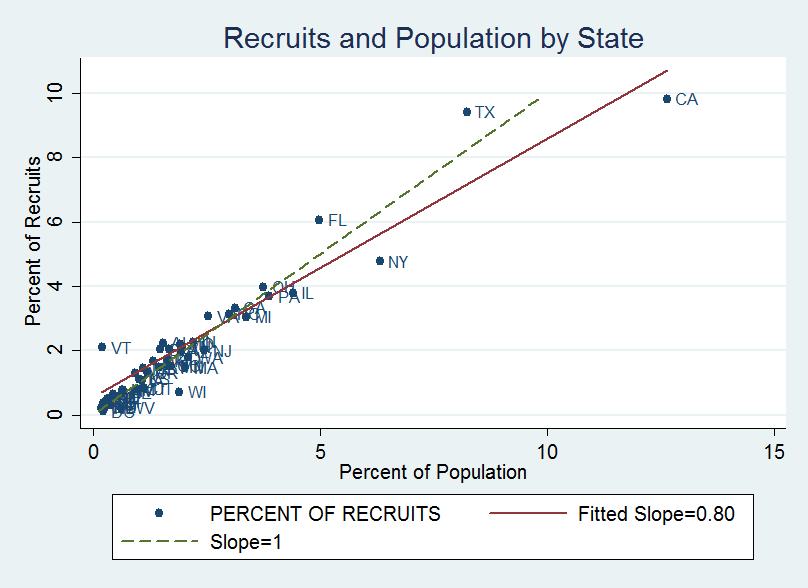
\includegraphics[scale=0.6]{../Output/graph_table1_rec_pop}
%\caption{State Percentage of Recruits by State Percentage of Young Male Population}
%\label{Flo: Figure: Recruits vs. Population}
%\end{figure}

%Graph of population percentage and death by state
%\begin{figure}
%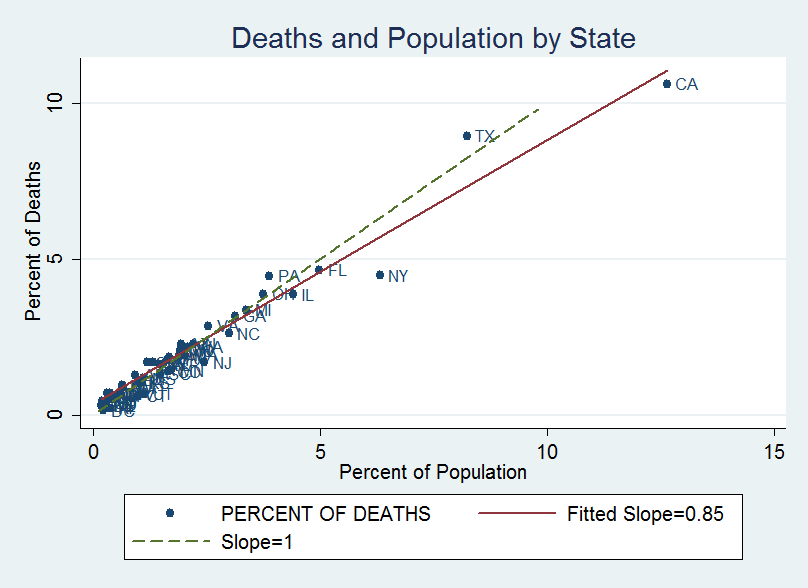
\includegraphics[scale=0.6]{../Output/graph_table1_death_pop}
%\caption{State Percentage of Population vs. State Percentage of Deaths}
%\label{Flo:Figure: Pop vs. Deaths}
%\end{figure}

\subsection {Additional Robustness Checks}
\paragraph{Other functional forms}
Economists often favor linear models in applied work, and these are shown in the main body of the paper, but some would consider Poisson regressions to be the most natural fit for count data with a large number of zeros that have no log, so I have exhaustively tested other models and find generally similar results across all specifications. I present these results here. 

Poisson regression fits a generalized linear model of the form $log(\mu_{i})=x'_{i}\beta$, so $\mu_{i}=exp(x'_{i}\beta)$ and a one unit increase in $x_{j}$ multiplies $\mu_{j}$ by $exp(\beta_{j})$. However, as I am modeling an underlying rate of enlistment, $\mu_{i}=e^{x'_{i}\beta}$, the observed number of recruits is the rate times the exposure, which in my case is the population of young males. If $R_{i}$ is the expected number of recruits, then $R_{i}=Population_{i}\cdot e^{x'_{i}\beta}=e^{ln(Population_{i})+x'_{i}\beta}$.
Thus all the Poisson models have been fitted with a coefficient constrained
to 1 for the county's log young male population.\footnote{Regressions without the offset give qualitatively similar results.} 

The detailed specification I estimate follows the equation: 
$$Recruits_{it}=Population_{i}\cdot e^{\beta_{0}Deaths_{i,t}+\beta_{1}Deaths_{i,t-1}+\beta_{2}Unemployment_{it}\\
+x'_{it}\eta+\alpha_{i}+\gamma_{t}+u_{it}}$$
where Deaths implies deaths from the given county, Unemployment county unemployment, and $x$ includes in-state (but out of county) deaths as well as
state unemployment. $\alpha_{i}$ is a set of fixed effects for each county, which flexibly control for any county characteristics such as the presence of a military base or political support for the military. $\gamma_{t}$ is a set of fixed effects for every month, so national characteristics that are the same across counties in any
given time period such as the total national number of deaths, national
unemployment rate, or the military wage rate are also flexibly controlled for and cannot be separately estimated. 

%Ordinary least squares results for recruit levels (as opposed to logs) are shown in Appendix Table \ref{Flo:County-basic}. All observations are weighted by county population. 
%Completely Linear Regression
%could be done now in redefined.do but no one cares
%\pagebreak{}
%\begin{table}
%\caption{}
%\label{Flo:County-basic}\includegraphics[bb=45bp 0bp 612bp 730bp,clip, scale=0.95]{../Output/PDF/redefW}
%\end{table}

 
%(I have
%run un-weighted regressions, in which the results are equally significant,
%if only about 1/3 as large). 

%One can see that with a full set of fixed effects, in-county deaths in the previous month are associated with 15 fewer applicants and nearly 10 fewer contracts. In-state deaths are associated with 0.3 to 1.1 fewer applicants, and 0.2 to 0.7 contracted recruits fewer, although the estimate is sometimes positive and not always statistically different from zero. The coefficient on lagged in-county deaths is the main estimate of interest, and is remarkably stable across different sets of fixed effects after county-level fixed effects are included.

%I have calculated, but do not show estimates of the elasticity of the recruiting response to death based on least squares regressions. They indicate that a one percent increase in the number of in-county deaths leads to a 2.7\% reduction in in-county recruits in the next month. However, I put less emphasis on this result for two reasons. First, the vast majority of county-months do not observe a death, and thus one cannot take the natural log of the data for simple elasticity calculations. Second, since most county-months have zero deaths, when any number of deaths is observed, there has actually been an infinite percent increase in the number of deaths. 

%There are of course methods to deal with the first problem and other ways to calculate elasticities, however the second reason makes the interpretation of the 2.7 coefficient fairly odd. It's hard to know what sort of effect is implied by a $2.7*\infty\%$ decrease in recruits. 
%Semi-elasticity estimates, where the right-hand side variable is in levels and the left hand side is logged eliminates some of the problems with logs of zero, but a non-trivial 30\% of county-months have zero active-duty recruits, so the log-linear OLS model is by no means ideal, even if it is more easily comparable to the Poisson estimates shown above.  One advantage of these linear models, however, is that I can test inclusion of state-by-year fixed effects which improves my case for causal identification. Unfortunately I cannot include these state-by-year fixed effects in Poisson regression due to convergence issues, however, the extra fixed effects result in similar estimates as the other specification; in some cases they make the effect appear even larger. 

Appendix Table \ref{Flo:Poisson Basic} shows the Poisson semi-elasticity estimates for both applicants and contracts. The dependent variable is active duty recruits. Observations have been weighted by county population. The semi-elasticity estimates show that an in-county death in the previous month leads to a 0.8 to 0.9\% reduction in both applicants and recruits, very similar to the log-linear regressions in the main body of the paper. Out-of-county deaths lead to small increases in recruiting.

%POISSON BASIC
%built by redefpoisson.do
\pagebreak{}
\begin{table}
\caption{Poisson Regressions of County Recruits on Deaths and Unemployment}
\label{Flo:Poisson Basic}
\scalebox{1}{\documentclass[]{article}
\setlength{\pdfpagewidth}{8.5in} \setlength{\pdfpageheight}{11in}
\begin{document}
\begin{tabular}{lcccccc} \hline
 & (1) & (2) & (3) & (4) & (5) & (6) \\
VARIABLES & Applicants & Applicants & Applicants & Contracts & Contracts & Contracts \\ \hline
 &  &  &  &  &  &  \\
Current In-County Deaths/100 & -0.045 & -0.180 & -0.089 & 0.027 & -0.146 & -0.086 \\
 & [0.436] & [0.433] & [0.320] & [0.448] & [0.431] & [0.310] \\
Lag In-County Deaths/100 & -0.756*** & -0.898*** & -0.793*** & -0.646** & -0.836*** & -0.774*** \\
 & [0.184] & [0.195] & [0.244] & [0.279] & [0.273] & [0.259] \\
Current Out-of-County Deaths/100 &  & 0.218*** & 0.183*** &  & 0.230*** & 0.139** \\
 &  & [0.064] & [0.062] &  & [0.070] & [0.071] \\
Lag Out-of-County Deaths/100 &  & 0.179*** & 0.155*** &  & 0.202*** & 0.103 \\
 &  & [0.066] & [0.058] &  & [0.078] & [0.064] \\
State Unemployment &  & -0.003 & -0.025*** &  & -0.010 & -0.025*** \\
 &  & [0.006] & [0.006] &  & [0.007] & [0.006] \\
County Unemployment &  & 0.016*** & 0.016*** &  & 0.016*** & 0.016*** \\
 &  & [0.005] & [0.004] &  & [0.005] & [0.004] \\
 &  &  &  &  &  &  \\
Observations & 178,239 & 178,169 & 178,169 & 178,182 & 178,112 & 178,112 \\
Number of fips & 3,127 & 3,127 & 3,127 & 3,126 & 3,126 & 3,126 \\
County FE & YES & YES & YES & YES & YES & YES \\
Month FE & YES & YES & YES & YES & YES & YES \\
State Trends & NO & NO & YES & NO & NO & YES \\
 Likelihood & -332831 & -331962 & -331200 & -278656 & -278173 & -277676 \\ \hline
\multicolumn{7}{c}{ Robust standard errors in brackets} \\
\multicolumn{7}{c}{ *** p$<$0.01, ** p$<$0.05, * p$<$0.1} \\
\multicolumn{7}{c}{ Notes: Table shows Poisson regression of national active duty recruits on deaths.} \\
\multicolumn{7}{c}{ Fixed effects are included separately by county and month, and linear state trends, as indiciated,} \\
\multicolumn{7}{c}{ The first four columns show applicants and the last three show contracts.} \\
\multicolumn{7}{c}{ Filename:redefPbasic.tex} \\
\end{tabular}
\end{document}
}
\end{table}

%Square Root
%\pagebreak{}
%\clearpage{}
%\begin{table}
%\caption{}
%\label{Flo:sqrt}
%\includegraphics[bb=45bp 0bp 612bp 730bp,clip,scale=0.95]{../Output/PDF/sqrt}
%\end{table}

%Negative Binomial
\pagebreak{}
\clearpage{}
\begin{table}
\caption{}
\label{Flo:negbinom}
\includegraphics[bb=45bp 0bp 612bp 730bp,clip,scale=0.95]{../Output/PDF/negbinom}
\end{table}

Additional specifications include modeling %the left hand side variable as 
with a negative binomial conditional fixed effects regression, with results shown in Table~\ref{Flo:negbinom}. Again, results are very similar: by far the largest deterrant effect comes from in-county deaths. Problems exist with negative binomial fixed effects regression, as explained in \cite{negbinom}, so these results are presented only to exhaustively test other functional forms and show that results are robust. 
%the square root of recruits, with results shown in Table~\ref{Flo:sqrt}, and

\paragraph{Tests of Additional Data}
In additionally to exhaustively testing functional forms and getting similarly robust results, I also obtain extremely similar results when I test only subsets on the data. For instance 
in addition to testing every recruit, I also test the model by using only deaths from active duty soldiers, as opposed to deaths of all soldiers (active, reserve, and guard) as in all other specification. Results, shown in Appendix Table~\ref{Flo:Rdeathslinear} appear slightly \textit{stronger}, in that deterrent effects of in-county deaths are estimated to be slightly larger than one percent. Appendix Table~\ref{Flo:RdeathsP} shows Poisson regressions using only active duty deaths and again, the results are robust

Tests of lead periods, i.e. testing the regression specification by testing for implausable effects of deaths in the future on current recruiting, are show in tables~\ref{Flo:forwardbasicLN} and~\ref{Flo:forwardPbasic}. The Poisson specification, as well as specifications using only active duty deaths, seem to pass this test.

%The main Poisson regression specification from Table~\ref{Flo:Poisson Basic} is repeated in Appendix Table~\ref{Flo:allrecruits} using all recruits, including the reserve and guard contracts that appear to be underreported in the FOIA data. Results are very similar. 


%Using Only Active Duty DEATHS (all the R variables)
%Linear. Have Poisson as well.
\pagebreak{}
\clearpage{}
\begin{table}
\caption{Active Duty Deaths Linear}
\label{Flo:Rdeathslinear}
\scalebox{0.9}{
\documentclass[]{article}
\setlength{\pdfpagewidth}{8.5in} \setlength{\pdfpageheight}{11in}
\begin{document}
\begin{tabular}{lcccccc}
\multicolumn{7}{c}{Log County Applicants vs Active Duty Deaths and Unemployment} \\ \hline
 & (1) & (2) & (3) & (4) & (5) & (6) \\
VARIABLES & Basic & State & w/Stateyear & Basic & State & w/Stateyear \\ \hline
 &  &  &  &  &  &  \\
In-County Active Duty Deaths/100 & -0.169 & -0.274 & -0.456 & -0.236 & -0.337 & -0.518 \\
 & [0.419] & [0.420] & [0.339] & [0.468] & [0.455] & [0.385] \\
Lag In-County Active Duty Deaths/100 & -1.294*** & -1.356*** & -1.525*** & -1.489*** & -1.512*** & -1.679*** \\
 & [0.314] & [0.326] & [0.307] & [0.382] & [0.417] & [0.462] \\
Out-of-County Active Duty Deaths &  & 0.153** & 0.125** &  & 0.180** & 0.169** \\
 &  & [0.074] & [0.064] &  & [0.075] & [0.077] \\
Lag Out-of-County Active Duty Deaths &  & 0.133* & 0.064 &  & 0.034 & -0.037 \\
 &  & [0.078] & [0.064] &  & [0.101] & [0.070] \\
County Unemployment &  & 0.013** & 0.011** &  & 0.015** & 0.013** \\
 &  & [0.005] & [0.005] &  & [0.006] & [0.005] \\
State Unemployment &  & 0.005 & -0.035*** &  & 0.001 & -0.030*** \\
 &  & [0.007] & [0.008] &  & [0.007] & [0.011] \\
 &  &  &  &  &  &  \\
Observations & 178,809 & 178,739 & 178,739 & 178,809 & 178,739 & 178,739 \\
R-squared & 0.964 & 0.965 & 0.965 & 0.956 & 0.957 & 0.958 \\
County FE & YES & YES & YES & YES & YES & YES \\
Month FE & YES & YES & YES & YES & YES & YES \\
 Stateyear FE & NO & NO & YES & NO & NO & YES \\ \hline
\multicolumn{7}{c}{ Robust standard errors in brackets} \\
\multicolumn{7}{c}{ *** p$<$0.01, ** p$<$0.05, * p$<$0.1} \\
\multicolumn{7}{c}{ Notes: Table shows linear regression estimates of log (national active duty recruits +1) on \textit{only} active duty deaths.} \\
\multicolumn{7}{c}{ Fixed effects are included separately by county and month, and for each state-year, as indiciated,} \\
\multicolumn{7}{c}{ The first three columns show applicants and the last three show contracts.} \\
\multicolumn{7}{c}{ Filename:LNLinearWR.tex} \\
\end{tabular}
\end{document}

}
%built in redefined.do
\end{table}


\begin{table}
%built in redefinedpoisson.do
\caption{Active Duty Deaths Poisson}
\label{Flo:RdeathsP} \documentclass[]{article}
\setlength{\pdfpagewidth}{8.5in} \setlength{\pdfpageheight}{11in}
\begin{document}
\begin{tabular}{lcccccc} \hline
 & (1) & (2) & (3) & (4) & (5) & (6) \\
VARIABLES & Applicants & Applicants & Applicants & Contracts & Contracts & Contracts \\ \hline
 &  &  &  &  &  &  \\
Active duty deaths this month-county & 0.002 & 0.000 & 0.002 & 0.002 & -0.001 & 0.000 \\
 & [0.004] & [0.005] & [0.004] & [0.005] & [0.005] & [0.004] \\
1 monthly lags of Rmonthcountydeath & -0.010*** & -0.012*** & -0.011*** & -0.009*** & -0.012*** & -0.011*** \\
 & [0.003] & [0.003] & [0.003] & [0.003] & [0.003] & [0.004] \\
R out of county but in-state deaths this month &  & 0.002*** & 0.002*** &  & 0.003*** & 0.002** \\
 &  & [0.001] & [0.001] &  & [0.001] & [0.001] \\
1 monthly lags of Routofcounty &  & 0.002*** & 0.002*** &  & 0.002** & 0.001 \\
 &  & [0.001] & [0.001] &  & [0.001] & [0.001] \\
State Unemployment &  & -0.002 & -0.025*** &  & -0.009 & -0.026*** \\
 &  & [0.006] & [0.006] &  & [0.006] & [0.006] \\
County Unemployment &  & 0.016*** & 0.016*** &  & 0.016*** & 0.016*** \\
 &  & [0.005] & [0.004] &  & [0.005] & [0.004] \\
 &  &  &  &  &  &  \\
Observations & 178,239 & 178,169 & 178,169 & 178,182 & 178,112 & 178,112 \\
Number of fips & 3,127 & 3,127 & 3,127 & 3,126 & 3,126 & 3,126 \\
County FE & YES & YES & YES & YES & YES & YES \\
Month FE & YES & YES & YES & YES & YES & YES \\
State Trends & NO & NO & YES & NO & NO & YES \\
 Likelihood & -332832 & -331963 & -331201 & -278655 & -278171 & -277676 \\ \hline
\multicolumn{7}{c}{ Robust standard errors in brackets} \\
\multicolumn{7}{c}{ *** p$<$0.01, ** p$<$0.05, * p$<$0.1} \\
\multicolumn{7}{c}{ Notes: Table shows Poisson regression of national active duty recruits on deaths.} \\
\multicolumn{7}{c}{ Fixed effects are included separately by county and month, and linear state trends, as indiciated,} \\
\multicolumn{7}{c}{ The first four columns show applicants and the last three show contracts.} \\
\multicolumn{7}{c}{ Filename:redefPbasicR.tex} \\
\end{tabular}
\end{document}

\end{table}


Appendix Tables~\ref{Flo:forwardbasicLN} and ~\ref{Flo:redefPF1} repeat the main specification but add lead periods of deaths as a falsification test of the model. As expected, deaths in the future have no relation to current recruiting. 


\clearpage{}
\begin{table}
%built by redefined.do
\caption{Testing Effect of Leads: Linear}
\label{Flo:forwardbasicLN}
\scalebox{0.8}{
\documentclass[]{article}
\setlength{\pdfpagewidth}{8.5in} \setlength{\pdfpageheight}{11in}
\begin{document}
\begin{tabular}{lcccccc} \hline
 & (1) & (2) & (3) & (4) & (5) & (6) \\
VARIABLES & Applicants & Applicants & Applicants & Contracts & Contracts & Contracts \\ \hline
 &  &  &  &  &  &  \\
Lead In-County Deaths/100 & -0.580** & -0.457* & -0.625*** & -0.758*** & -0.627** & -0.821*** \\
 & [0.228] & [0.269] & [0.234] & [0.259] & [0.292] & [0.265] \\
Current In-County Deaths/100 & -0.533* & -0.525 & -0.627** & -0.537** & -0.485 & -0.622** \\
 & [0.281] & [0.360] & [0.270] & [0.250] & [0.356] & [0.249] \\
Lag In-County Deaths/100 & -1.092*** & -1.065*** & -1.199*** & -1.180*** & -1.114*** & -1.248*** \\
 & [0.218] & [0.194] & [0.227] & [0.276] & [0.248] & [0.290] \\
Lead Out-of-County Deaths/100 &  & 0.097 & 0.042 &  & 0.074 & 0.048 \\
 &  & [0.059] & [0.061] &  & [0.062] & [0.072] \\
Current Out-of-County Deaths/100 &  & 0.149** & 0.130** &  & 0.162** & 0.129* \\
 &  & [0.059] & [0.055] &  & [0.066] & [0.068] \\
Lag Out-of-County Deaths/100 &  & 0.101 & 0.044 &  & 0.007 & -0.049 \\
 &  & [0.066] & [0.058] &  & [0.082] & [0.069] \\
State Unemployment &  & 0.003 & -0.035*** &  & -0.000 & -0.031*** \\
 &  & [0.007] & [0.008] &  & [0.008] & [0.011] \\
County Unemployment &  & 0.013** & 0.011** &  & 0.015** & 0.013** \\
 &  & [0.006] & [0.005] &  & [0.006] & [0.005] \\
 &  &  &  &  &  &  \\
Observations & 175,672 & 175,602 & 175,602 & 175,672 & 175,602 & 175,602 \\
R-squared & 0.965 & 0.965 & 0.965 & 0.958 & 0.957 & 0.958 \\
County FE & YES & YES & YES & YES & YES & YES \\
Month FE & YES & YES & YES & YES & YES & YES \\
 Stateyear FE & NO & NO & YES & NO & NO & YES \\ \hline
\multicolumn{7}{c}{ Robust standard errors in brackets} \\
\multicolumn{7}{c}{ *** p$<$0.01, ** p$<$0.05, * p$<$0.1} \\
\multicolumn{7}{c}{ Notes: Table shows linear regression estimates of log (national active duty recruits +1) on deaths} \\
\multicolumn{7}{c}{ As well as future 'lead' periods. Fixed effects are included separately by county and month, and for each state-year, as indiciated,} \\
\multicolumn{7}{c}{ The first columns show applicants and the last show contracts.} \\
\multicolumn{7}{c}{ Filename:forwardbasicWLN.txt} \\
\end{tabular}
\end{document}
}
\end{table}

%Future Deaths Have No Effect
%built by redefinedpoisson.do
\pagebreak{}
\clearpage{}
\begin{table}
\caption{Testing Effect of Leads: Poisson}
\label{Flo:forwardPbasic}
\scalebox{0.9}{
\documentclass[]{article}
\setlength{\pdfpagewidth}{8.5in} \setlength{\pdfpageheight}{11in}
\begin{document}
\begin{tabular}{lcccccc} \hline
 & (1) & (2) & (3) & (4) & (5) & (6) \\
VARIABLES & Applicants & Applicants & Applicants & Contracts & Contracts & Contracts \\ \hline
 &  &  &  &  &  &  \\
Lead In-County Deaths/100 & -0.047 & -0.172 & -0.084 & -0.042 & -0.170 & -0.121 \\
 & [0.268] & [0.289] & [0.267] & [0.313] & [0.317] & [0.262] \\
Current In-County Deaths/100 & -0.120 & -0.287 & -0.195 & -0.034 & -0.209 & -0.156 \\
 & [0.402] & [0.417] & [0.328] & [0.425] & [0.431] & [0.335] \\
Lag In-County Deaths/100 & -0.680*** & -0.846*** & -0.761*** & -0.583** & -0.758*** & -0.721** \\
 & [0.175] & [0.190] & [0.258] & [0.238] & [0.250] & [0.283] \\
Lead Out-of-County Deaths/100 &  & 0.126** & 0.097 &  & 0.120* & 0.042 \\
 &  & [0.059] & [0.067] &  & [0.064] & [0.065] \\
Current Out-of-County Deaths/100 &  & 0.188*** & 0.188*** &  & 0.202*** & 0.143** \\
 &  & [0.060] & [0.060] &  & [0.067] & [0.069] \\
Lag Out-of-County Deaths/100 &  & 0.180*** & 0.164*** &  & 0.191** & 0.113* \\
 &  & [0.063] & [0.058] &  & [0.075] & [0.064] \\
State Unemployment & -0.006 & -0.004 & -0.030*** & -0.012* & -0.011* & -0.030*** \\
 & [0.006] & [0.006] & [0.006] & [0.007] & [0.006] & [0.006] \\
County Unemployment & 0.016*** & 0.016*** & 0.018*** & 0.016*** & 0.016*** & 0.018*** \\
 & [0.005] & [0.005] & [0.004] & [0.005] & [0.005] & [0.004] \\
 &  &  &  &  &  &  \\
Observations & 174,986 & 174,986 & 174,986 & 174,986 & 174,986 & 174,986 \\
Number of fips & 3,126 & 3,126 & 3,126 & 3,126 & 3,126 & 3,126 \\
County FE & YES & YES & YES & YES & YES & YES \\
Month FE & YES & YES & YES & YES & YES & YES \\
Stateyear FE & NO & NO & YES & NO & NO & YES \\
 Likelihood & -325865 & -325835 & -325360 & -272927 & -272907 & -272543 \\ \hline
\multicolumn{7}{c}{ Robust standard errors in brackets} \\
\multicolumn{7}{c}{ *** p$<$0.01, ** p$<$0.05, * p$<$0.1} \\
\multicolumn{7}{c}{ Notes: Table shows Poisson regression of national active duty recruits on deaths} \\
\multicolumn{7}{c}{ As well as future 'lead' periods. Fixed effects are included separately by county and month} \\
\multicolumn{7}{c}{ and for each state-year, as indiciated, as well as a state-specific linear trend.} \\
\multicolumn{7}{c}{ The first four columns show applicants and the last four show contracts.} \\
\multicolumn{7}{c}{ Filename:forwardPbasic.txt} \\
\end{tabular}
\end{document}
}
\end{table}


I also use additional data on deaths acquired through a FOIA request. This data consists of all deaths of anyone in the military from 1990-2006, regardless of circumstance or location. Thus it includes numerous deaths that are completely unrelated to the wars in Iraq or Afghanistan, and even unrelated to the military---heart attacks, car accidents, etc. As I expected given the comparatively banal circumstances of the majority of these deaths, all regressions indicate no significant recruiting response to in-county deaths, neither in the entire 1990-2006 period nor the 2001-2006 period used in the main regression tables. These results are shown in Appendix Table~\ref{Flo:LNlinear90}.% and ~\ref{Flo:alldeaths90}.

%Non-Combat Deaths, 1990-2006
%buily by PandLN90.do
\begin{table}
\caption{}
\label{Flo:LNlinear90}
\scalebox{0.8}{
\input{../Output/LNlinear90.tex}}
\end{table}

%Works, but why bother?
%\begin{table}
%\caption{}
%\label{Flo:alldeaths90}
%\scalebox{0.8}{
%\documentclass[]{article}
\setlength{\pdfpagewidth}{8.5in} \setlength{\pdfpageheight}{11in}
\begin{document}
\begin{tabular}{lcccc} \hline
 & (1) & (2) & (3) & (4) \\
VARIABLES & Applicants & Applicants & Applicants & Contracts \\ \hline
 &  &  &  &  \\
In-County Deaths/100 & 0.339 & 0.321 & 0.091 & 0.471 \\
 & [0.379] & [0.369] & [0.279] & [0.375] \\
Lag In-County Deaths/100 & 0.371 & 0.359 & 0.113 & 0.277 \\
 & [0.401] & [0.392] & [0.315] & [0.398] \\
Out-of-County Deaths/100 &  & 0.268*** & -0.025 &  \\
 &  & [0.052] & [0.041] &  \\
Lag Out-of-County Deaths/100 &  & 0.247*** & -0.014 &  \\
 &  & [0.047] & [0.038] &  \\
State Unemployment &  & 0.006 & 0.022*** &  \\
 &  & [0.004] & [0.004] &  \\
County Unemployment &  & 0.014*** & 0.015*** &  \\
 &  & [0.002] & [0.001] &  \\
 &  &  &  &  \\
Observations & 619,542 & 619,425 & 619,425 & 619,542 \\
Number of fips & 3,129 & 3,129 & 3,129 & 3,129 \\
County FE & YES & YES & YES & YES \\
Month FE & YES & YES & YES & YES \\
State Trends & NO & NO & YES & NO \\
 Likelihood & -1.293e+06 & -1.291e+06 & -1.279e+06 & -1.047e+06 \\ \hline
\multicolumn{5}{c}{ Robust standard errors in brackets} \\
\multicolumn{5}{c}{ *** p$<$0.01, ** p$<$0.05, * p$<$0.1} \\
\multicolumn{5}{c}{ Notes: Table shows Poisson regression estimates of national active duty recruits on deaths.} \\
\multicolumn{5}{c}{ Fixed effects are included separately by county and month, and linear state trends, as indiciated,} \\
\multicolumn{5}{c}{ The first four columns show applicants and the last three show contracts.} \\
\multicolumn{5}{c}{ Filename:redefPbasic.tex} \\
\end{tabular}
\end{document}
}
%\end{table}

Tests of the entire set of recruits (active duty, guard, and reserve troops, not just active duty recruits as are used in most specifications) reveal similarly robust results--the deterrent effect appears even larger under this specification. Results are shown in Appendix Table~\ref{Flo:allrecruits}.

%made in redefined.do on 7/26/2016
\begin{table}
\caption{}
\label{Flo:allrecruits}
\scalebox{0.8}{
\documentclass[]{article}
\setlength{\pdfpagewidth}{8.5in} \setlength{\pdfpageheight}{11in}
\begin{document}
\begin{tabular}{lcccccc}
\multicolumn{7}{c}{Log County ALL Applicants vs Deaths and Unemployment} \\ \hline
 & (1) & (2) & (3) & (4) & (5) & (6) \\
VARIABLES & Basic & State & w/Stateyear & Basic & State & w/Stateyear \\ \hline
 &  &  &  &  &  &  \\
Current In-County Deaths/100 & -0.360 & -0.452 & -0.593*** & -0.376 & -0.453 & -0.598** \\
 & [0.328] & [0.327] & [0.192] & [0.361] & [0.350] & [0.235] \\
Lag In-County Deaths/100 & -1.141*** & -1.179*** & -1.275*** & -1.140*** & -1.178*** & -1.265*** \\
 & [0.185] & [0.198] & [0.207] & [0.233] & [0.238] & [0.285] \\
Current Out-of-County Deaths/100 &  & 0.215*** & 0.156*** &  & 0.165** & 0.130* \\
 &  & [0.057] & [0.048] &  & [0.067] & [0.069] \\
Lag Out-of-County Deaths/100 &  & 0.065 & 0.009 &  & 0.016 & -0.036 \\
 &  & [0.062] & [0.049] &  & [0.084] & [0.068] \\
County Unemployment &  & 0.018*** & 0.016*** &  & 0.015** & 0.013** \\
 &  & [0.005] & [0.004] &  & [0.006] & [0.005] \\
State Unemployment &  & 0.007 & -0.043*** &  & -0.000 & -0.031*** \\
 &  & [0.007] & [0.007] &  & [0.007] & [0.011] \\
 &  &  &  &  &  &  \\
Observations & 178,809 & 178,739 & 178,739 & 178,809 & 178,739 & 178,739 \\
R-squared & 0.969 & 0.970 & 0.971 & 0.957 & 0.957 & 0.958 \\
County FE & YES & YES & YES & YES & YES & YES \\
Month FE & YES & YES & YES & YES & YES & YES \\
 Stateyear FE & NO & NO & YES & NO & NO & YES \\ \hline
\multicolumn{7}{c}{ Robust standard errors in brackets} \\
\multicolumn{7}{c}{ *** p$<$0.01, ** p$<$0.05, * p$<$0.1} \\
\multicolumn{7}{c}{ Notes: Table shows linear regression estimates of log (national recruits +1) on military deaths.} \\
\multicolumn{7}{c}{ Fixed effects are included separately by county and month, and for each state-year, as indiciated,} \\
\multicolumn{7}{c}{ The first three columns show applicants and the last three show contracts.} \\
\multicolumn{7}{c}{ Filename:allrecLNLinearW.tex} \\
\end{tabular}
\end{document}
}
\end{table}

Tests of the heterogeneity of the effect by which the war in which the death occur also appear significantly stronger using a Poisson regression. Results are shown in Appendix Table~\ref{Flo:Deaths by WarP}.

\begin{table}
\caption{Deaths by War, Poisson}
\label{Flo:Deaths by WarP}
\documentclass[]{article}
\setlength{\pdfpagewidth}{8.5in} \setlength{\pdfpageheight}{11in}
\begin{document}
\begin{tabular}{lcccc} \hline
 & (1) & (2) & (3) & (4) \\
VARIABLES & Applicants & Applicants & Contracts & Contracts \\ \hline
 &  &  &  &  \\
In-County Deaths/100 & -0.044 & -0.047 & -0.068 & -0.071 \\
 & [0.315] & [0.316] & [0.310] & [0.310] \\
Iraq Lag In-County Deaths/100 & -0.839*** & -0.848*** & -0.778*** & -0.790*** \\
 & [0.306] & [0.312] & [0.281] & [0.281] \\
Afghanistan Lag In-County Deaths/100 & 1.270 & 1.199 & 0.734 & 0.735 \\
 & [0.898] & [0.909] & [1.155] & [1.148] \\
Out-of-County Deaths/100 & 0.183*** & 0.179*** & 0.139** & 0.133* \\
 & [0.062] & [0.061] & [0.071] & [0.070] \\
Iraq Lag Out-of-County Deaths/100 &  & 0.170*** &  & 0.126** \\
 &  & [0.059] &  & [0.063] \\
Afghanistan Lag Out-of-County Deaths/100 &  & -0.334 &  & -0.145 \\
 &  & [0.240] &  & [0.232] \\
State Unemployment & -0.024*** & -0.025*** & -0.025*** & -0.025*** \\
 & [0.006] & [0.005] & [0.006] & [0.006] \\
County Unemployment & 0.016*** & 0.016*** & 0.016*** & 0.016*** \\
 & [0.004] & [0.004] & [0.004] & [0.004] \\
Lag Out-of-County Deaths/100 & 0.162*** &  & 0.107* &  \\
 & [0.059] &  & [0.064] &  \\
 &  &  &  &  \\
Observations & 178,169 & 178,169 & 178,112 & 178,112 \\
Number of fips & 3,127 & 3,127 & 3,126 & 3,126 \\
County FE & YES &  & YES &  \\
Month FE & YES &  & YES &  \\
State Trend FE & YES &  & YES &  \\
Likelihood & -331198 & -331195 & -277676 & -277675 \\
Test & 0.0380 &  & 0.205 &  \\
State &  & 0.0377 &  & 0.240 \\
 County &  & 0.0487 &  & 0.198 \\ \hline
\multicolumn{5}{c}{ Robust standard errors in brackets} \\
\multicolumn{5}{c}{ *** p$<$0.01, ** p$<$0.05, * p$<$0.1} \\
\multicolumn{5}{c}{ Notes: Table shows Poisson regression estimates of national active duty recruits on deaths} \\
\multicolumn{5}{c}{ from different wars. Fixed effects are included separately by county and month as indiciated,} \\
\multicolumn{5}{c}{ The first two columns show applicants and the last two show contracts.} \\
\multicolumn{5}{c}{ Filename:redefPwar.tex} \\
\end{tabular}
\end{document}

\end{table}

%\subsection{Recruits and Deaths Across Service Branches}
%In this section I examine how the individual services fare in their recruiting. There are clearly differences between the services in terms of their operations; perhaps stemming from this there are often assumed to be significant cultural differences between the branches, leading to a difference in the type of people who make up the potential applicant pool for each of the services, and the possibility for a difference in the potential applicants' response to a local death.

%Table \ref{Flo:Recruits by Service} shows these estimates, again using Poisson regression analysis at the month-county level, with county and monthly fixed effects and state time trends. It appears that Marine recruiting decreases at a rate of over 2\% for every death, while the Air Force reaction to death is a statistically insignificant 0.05\% reduction in recruits. Deaths at the state level and state and county unemployment seem to have effects that are less clearly distinguishable across service branches. This makes sense given that very few of the deaths in Iraq and Afghanistan have come from the Air Force, while many have come from the Marines. But an even larger proportion have come from the Army, so if potential recruits were simply steeringaway from the branches of the military with the most deaths, the Army would be the branch with the largest recruiting response to deaths, which is not the case. I have repeated this exercise using weighted least squares regressions of the log of the recruits of each service branch, and the deterrent effects by service branch maintain the same ratios relative to one another, exhibiting further evidence that the recruiting deterrent is greatest for the Marine Corps. 
% Break recruits out by service branch
%\pagebreak{}
%\clearpage{}
%\begin{table}
%\caption{}
%\label{Flo:Recruits by Service}\includegraphics[bb=45bp 0bp 612bp 730bp,clip, scale=0.91]{../Output/PDF/highqualitybyserviceP}
%\end{table}

%Amongst the four branches of the military, the deaths in Iraq and Afghanistan have been highly concentrated amongst soldiers in the Army and the Marines. In the data used in this paper, roughly 2000 deaths are from the Army, 800 from the Marines, 85 from the Navy, and 50 from the Air Force. Since there have been 40 times more deaths in the Army than the Air Force, it is entirely possible that potential Army recruits have instead gone on to join the Air Force instead.

%To test this, I have rearranged the data into county-month-service branch observations and test the recruiting response to a specific service branch after deaths from the same service branch and from other service branches. Table \ref{Flo:Death by Same-Service Other-Service} shows the results of these tests. Poisson regressions shows the percent response to a death in the same service branch as the recruit, and in any of the other three service branches. As before, I have controlled for monthly fixed effects, state trends, and state and county unemployment.
%In these regressions I have included interacted county{*}service branch fixed effects as well. The bottom of the table shows pair-wise comparisons of the corresponding same-service and other-service death coefficients. For example, for applicants, a lagged same-service in-county death leads to a 0.7\% reduction in recruits in that service, while a lagged other-service in-county death leads to a 1.1\% reduction in recruits for that service. In all of the specifications, tests fail to reject the hypothesis that the effect of a lagged same-service in-county death is statistically identical to that of a lagged other-service in-county death. The same can be said of lagged same-service out-of-county deaths and lagged other-service out-of-county deaths. However, for several of the current-month deaths, statistical tests reject equivalence.
%They indicate that same-service deaths have a larger (and positive effect) than do other-service deaths. \emph{A priori} I would have assumed that if anything, same-service deaths would lead to a larger decrease in recruits, since recruits could either not sign up or substitute to a different service, but this does not seem to be the case. The results are further evidence that potential recruits are not using the information contained in a death (in this case, the service branch in which the death occurred) in a sophisticated or strictly risk-based manner.

%A slightly different way to get at the question of deaths by service branch is to lump all the recruits together but show the specific  response to deaths in a given service. These estimates are shown in Table \ref{Flo: Death by Service}. The coefficients are positive for Air Force and the Navy in-county deaths, however they are not statistically significant. I have also run specifications with the in-state but out-of-county deaths split by service branch, and I have run tests of equivalence of the coefficients for all the service branches. The hypotheses of equality cannot be rejected for county deaths, butcan be for state deaths. 




%POISSON RECRUITER AND MORTALITY CONTROLS
%\clearpage{}
%\pagebreak{}
%\begin{table}
%\caption{DO IN LOG LINEAR!!!}
%\label{Flo:Poisson Rec&Mort}\includegraphics[bb=45bp 0bp 612bp 730bp,clip,scale=0.95]{../Output/PDF/redefPrec}
%\end{table}

%MEDIA MARKET AND CONTIGUOUS-IN POISSON
%built by redefcontig.do
%\pagebreak{}
%\begin{table}
%\caption{Poisson version of media and neighboring}
%\label{Flo:Media}\includegraphics[bb=45bp 0bp 612bp 730bp,clip, scale=0.91]{../Output/PDF/redefcontigP}
%\end{table}

%POISSON Cumulative Lags
%\clearpage{}
%\pagebreak{}
%\begin{table}
%\caption{}
%\label{Flo:Cumulative LagsP}\input{../Output/redefrunninglagsP}
%\end{table}

%POISSON INTERACTIONS
%\clearpage{}
%\pagebreak{}
%\begin{table}
%\caption{Interactions in Poisson}
%\label{Flo:Poisson Interactions}\includegraphics[bb=45bp 0bp 612bp 730bp,clip,scale=0.95]{../Output/PDF/redefPinteractions}
%\end{table}

%POISSON QUALITY OF RECRUIT
%\pagebreak{}
%\begin{table}
%\caption{}
%\label{Flo: Recs by QualityP}\documentclass[]{article}
\setlength{\pdfpagewidth}{8.5in} \setlength{\pdfpageheight}{11in}
\begin{document}
\begin{tabular}{lcccccccc} \hline
 & (1) & (2) & (3) & (4) & (5) & (6) & (7) & (8) \\
VARIABLES & RLQmonthcounty & RHQ50monthcounty & RHQ50altmonthcounty & RHQ75monthcounty & RLQmonthcounty & RHQ50monthcounty & RHQ50altmonthcounty & RHQ75monthcounty \\ \hline
 &  &  &  &  &  &  &  &  \\
In-County Deaths/100 & -0.126 & -0.270 & 0.056 & -0.729 & -0.330 & 0.091 & 0.270 & 2.155 \\
 & [0.450] & [0.508] & [0.526] & [1.070] & [0.443] & [0.468] & [0.484] & [1.363] \\
Lag In-County Deaths/100 & -0.943*** & -0.824*** & -0.809*** & -2.861*** & -1.058*** & -0.545 & -0.880*** & -2.685 \\
 & [0.284] & [0.299] & [0.213] & [0.867] & [0.321] & [0.362] & [0.307] & [1.738] \\
Out-of-County Deaths/100 & 0.230*** & 0.194** & 0.231*** & 0.382 & 0.236*** & 0.216** & 0.226*** & 0.430 \\
 & [0.080] & [0.090] & [0.074] & [0.303] & [0.091] & [0.091] & [0.078] & [0.348] \\
Lag Out-of-County Deaths/100 & 0.139* & 0.249*** & 0.326*** & 0.105 & 0.153 & 0.264*** & 0.276*** & 0.066 \\
 & [0.079] & [0.085] & [0.078] & [0.266] & [0.102] & [0.097] & [0.090] & [0.356] \\
State Unemployment & -0.011 & 0.009 & 0.009 & 0.013 & -0.021*** & 0.005 & 0.004 & -0.008 \\
 & [0.007] & [0.007] & [0.007] & [0.017] & [0.007] & [0.008] & [0.007] & [0.020] \\
County Unemployment & 0.013*** & 0.024*** & 0.013*** & 0.013 & 0.011** & 0.025*** & 0.015*** & 0.023** \\
 & [0.005] & [0.006] & [0.004] & [0.010] & [0.004] & [0.006] & [0.005] & [0.011] \\
month==200112 & -0.053*** & -0.078*** & -0.060*** & -0.113** & -0.071*** & -0.034* & -0.033** & -0.118* \\
 & [0.013] & [0.016] & [0.012] & [0.055] & [0.014] & [0.018] & [0.013] & [0.069] \\
month==200201 & 0.184*** & 0.280*** & 0.204*** & 0.221*** & 0.154*** & 0.211*** & 0.171*** & 0.095 \\
 & [0.012] & [0.015] & [0.012] & [0.052] & [0.014] & [0.018] & [0.013] & [0.065] \\
month==200202 & 0.067*** & 0.069*** & 0.039*** & 0.079 & 0.101*** & 0.095*** & 0.082*** & -0.018 \\
 & [0.012] & [0.016] & [0.013] & [0.059] & [0.014] & [0.018] & [0.014] & [0.064] \\
month==200203 & 0.087*** & 0.027 & 0.016 & 0.143*** & 0.191*** & 0.052*** & 0.088*** & 0.051 \\
 & [0.013] & [0.017] & [0.013] & [0.052] & [0.013] & [0.019] & [0.014] & [0.067] \\
month==200204 & 0.097*** & 0.052*** & 0.024* & 0.121** & 0.150*** & 0.065*** & 0.067*** & 0.113* \\
 & [0.013] & [0.015] & [0.012] & [0.051] & [0.014] & [0.017] & [0.013] & [0.061] \\
month==200205 & 0.016 & 0.083*** & -0.021* & 0.171*** & -0.014 & 0.111*** & 0.022 & 0.184*** \\
 & [0.013] & [0.016] & [0.012] & [0.052] & [0.014] & [0.018] & [0.014] & [0.062] \\
month==200206 & 0.156*** & 0.284*** & 0.206*** & 0.265*** & 0.159*** & 0.289*** & 0.218*** & 0.182*** \\
 & [0.015] & [0.015] & [0.014] & [0.053] & [0.016] & [0.018] & [0.015] & [0.063] \\
month==200207 & 0.220*** & 0.371*** & 0.286*** & 0.345*** & 0.221*** & 0.391*** & 0.308*** & 0.304*** \\
 & [0.013] & [0.015] & [0.012] & [0.053] & [0.014] & [0.016] & [0.013] & [0.060] \\
month==200208 & 0.169*** & 0.298*** & 0.208*** & 0.283*** & 0.228*** & 0.393*** & 0.308*** & 0.279*** \\
 & [0.013] & [0.015] & [0.012] & [0.054] & [0.013] & [0.017] & [0.013] & [0.059] \\
month==200209 & 0.124*** & 0.223*** & 0.160*** & 0.249*** & 0.231*** & 0.399*** & 0.326*** & 0.329*** \\
 & [0.013] & [0.015] & [0.013] & [0.051] & [0.014] & [0.016] & [0.013] & [0.059] \\
month==200210 & 0.099*** & 0.158*** & 0.146*** & 0.212*** & 0.051*** & 0.112*** & 0.090*** & 0.112* \\
 & [0.013] & [0.015] & [0.013] & [0.054] & [0.015] & [0.017] & [0.014] & [0.067] \\
month==200211 & -0.017 & -0.043*** & 0.001 & -0.052 & 0.027* & 0.013 & 0.051*** & -0.018 \\
 & [0.012] & [0.015] & [0.012] & [0.059] & [0.014] & [0.017] & [0.013] & [0.063] \\
month==200212 & -0.112*** & -0.108*** & -0.093*** & -0.032 & -0.106*** & -0.093*** & -0.081*** & -0.052 \\
 & [0.013] & [0.017] & [0.013] & [0.056] & [0.014] & [0.019] & [0.014] & [0.062] \\
month==200301 & 0.014 & 0.216*** & 0.129*** & 0.376*** & -0.020 & 0.138*** & 0.102*** & 0.200*** \\
 & [0.013] & [0.016] & [0.013] & [0.048] & [0.015] & [0.018] & [0.015] & [0.060] \\
month==200302 & -0.163*** & 0.013 & -0.042*** & 0.244*** & -0.151*** & 0.010 & -0.017 & 0.154** \\
 & [0.014] & [0.016] & [0.014] & [0.055] & [0.016] & [0.019] & [0.015] & [0.060] \\
month==200303 & -0.020 & 0.172*** & 0.088*** & 0.406*** & -0.091*** & 0.097*** & 0.063*** & 0.248*** \\
 & [0.015] & [0.016] & [0.013] & [0.052] & [0.016] & [0.019] & [0.016] & [0.064] \\
month==200304 & -0.032** & 0.293*** & 0.154*** & 0.593*** & -0.095*** & 0.209*** & 0.129*** & 0.450*** \\
 & [0.015] & [0.016] & [0.014] & [0.051] & [0.017] & [0.018] & [0.016] & [0.058] \\
month==200305 & -0.155*** & 0.115*** & -0.039*** & 0.367*** & -0.139*** & 0.176*** & 0.045*** & 0.396*** \\
 & [0.014] & [0.016] & [0.014] & [0.053] & [0.015] & [0.019] & [0.015] & [0.060] \\
month==200306 & 0.053*** & 0.309*** & 0.212*** & 0.385*** & 0.003 & 0.337*** & 0.237*** & 0.345*** \\
 & [0.016] & [0.017] & [0.015] & [0.054] & [0.016] & [0.020] & [0.016] & [0.061] \\
month==200307 & 0.042*** & 0.287*** & 0.196*** & 0.340*** & 0.073*** & 0.331*** & 0.267*** & 0.231*** \\
 & [0.015] & [0.016] & [0.014] & [0.055] & [0.015] & [0.018] & [0.014] & [0.061] \\
month==200308 & -0.018 & 0.209*** & 0.125*** & 0.199*** & 0.007 & 0.294*** & 0.224*** & 0.193*** \\
 & [0.015] & [0.016] & [0.014] & [0.054] & [0.015] & [0.019] & [0.016] & [0.061] \\
month==200309 & -0.059*** & 0.090*** & 0.023* & 0.141*** & -0.004 & 0.225*** & 0.149*** & 0.230*** \\
 & [0.013] & [0.016] & [0.013] & [0.054] & [0.015] & [0.019] & [0.015] & [0.063] \\
month==200310 & -0.055*** & 0.040*** & 0.038*** & 0.029 & -0.132*** & 0.054*** & 0.036*** & -0.018 \\
 & [0.014] & [0.015] & [0.013] & [0.055] & [0.015] & [0.018] & [0.014] & [0.064] \\
month==200311 & -0.283*** & -0.221*** & -0.193*** & -0.259*** & -0.271*** & -0.127*** & -0.123*** & -0.129* \\
 & [0.014] & [0.017] & [0.014] & [0.061] & [0.016] & [0.021] & [0.016] & [0.069] \\
month==200312 & -0.252*** & -0.157*** & -0.147*** & -0.096 & -0.243*** & -0.102*** & -0.096*** & -0.029 \\
 & [0.014] & [0.016] & [0.014] & [0.061] & [0.016] & [0.018] & [0.015] & [0.064] \\
month==200401 & -0.127*** & 0.071*** & 0.004 & 0.058 & -0.147*** & 0.072*** & 0.034** & 0.067 \\
 & [0.013] & [0.016] & [0.013] & [0.058] & [0.015] & [0.020] & [0.016] & [0.067] \\
month==200402 & -0.212*** & -0.075*** & -0.091*** & 0.020 & -0.180*** & -0.016 & -0.020 & -0.019 \\
 & [0.014] & [0.018] & [0.014] & [0.057] & [0.016] & [0.020] & [0.015] & [0.065] \\
month==200403 & -0.089*** & 0.056*** & 0.020 & 0.195*** & -0.083*** & 0.062*** & 0.063*** & 0.126* \\
 & [0.014] & [0.016] & [0.013] & [0.055] & [0.016] & [0.018] & [0.015] & [0.065] \\
month==200404 & -0.178*** & -0.049*** & -0.109*** & 0.039 & -0.096*** & 0.013 & -0.009 & 0.042 \\
 & [0.014] & [0.018] & [0.014] & [0.057] & [0.017] & [0.019] & [0.016] & [0.069] \\
month==200405 & -0.348*** & -0.142*** & -0.265*** & 0.104* & -0.296*** & -0.127*** & -0.207*** & 0.024 \\
 & [0.015] & [0.018] & [0.015] & [0.056] & [0.016] & [0.021] & [0.017] & [0.062] \\
month==200406 & -0.132*** & 0.081*** & 0.002 & 0.106* & -0.147*** & 0.077*** & 0.005 & -0.022 \\
 & [0.015] & [0.016] & [0.014] & [0.055] & [0.017] & [0.019] & [0.016] & [0.065] \\
month==200407 & -0.208*** & -0.042** & -0.124*** & -0.066 & -0.169*** & 0.035* & -0.016 & -0.129* \\
 & [0.015] & [0.019] & [0.014] & [0.059] & [0.016] & [0.021] & [0.016] & [0.074] \\
month==200408 & -0.201*** & -0.002 & -0.110*** & 0.115** & -0.174*** & 0.083*** & -0.016 & 0.019 \\
 & [0.014] & [0.016] & [0.014] & [0.054] & [0.015] & [0.020] & [0.016] & [0.061] \\
month==200409 & -0.249*** & -0.163*** & -0.256*** & -0.108** & -0.221*** & -0.047** & -0.136*** & -0.020 \\
 & [0.015] & [0.018] & [0.016] & [0.054] & [0.016] & [0.019] & [0.015] & [0.066] \\
month==200410 & -0.282*** & -0.239*** & -0.269*** & -0.161*** & -0.335*** & -0.230*** & -0.260*** & -0.208*** \\
 & [0.015] & [0.017] & [0.014] & [0.057] & [0.017] & [0.020] & [0.015] & [0.068] \\
month==200411 & -0.333*** & -0.207*** & -0.229*** & -0.113* & -0.443*** & -0.276*** & -0.272*** & -0.297*** \\
 & [0.014] & [0.019] & [0.015] & [0.059] & [0.018] & [0.020] & [0.016] & [0.072] \\
month==200412 & -0.399*** & -0.291*** & -0.333*** & -0.133** & -0.441*** & -0.286*** & -0.317*** & -0.270*** \\
 & [0.016] & [0.020] & [0.016] & [0.059] & [0.018] & [0.020] & [0.017] & [0.067] \\
month==200501 & -0.310*** & -0.070*** & -0.178*** & 0.011 & -0.375*** & -0.117*** & -0.181*** & -0.191*** \\
 & [0.015] & [0.018] & [0.015] & [0.057] & [0.017] & [0.022] & [0.017] & [0.071] \\
month==200502 & -0.429*** & -0.306*** & -0.372*** & -0.137** & -0.376*** & -0.254*** & -0.290*** & -0.178** \\
 & [0.015] & [0.019] & [0.015] & [0.055] & [0.018] & [0.021] & [0.017] & [0.070] \\
month==200503 & -0.210*** & -0.152*** & -0.211*** & 0.070 & -0.265*** & -0.154*** & -0.185*** & -0.074 \\
 & [0.015] & [0.017] & [0.014] & [0.055] & [0.017] & [0.021] & [0.015] & [0.068] \\
month==200504 & -0.302*** & -0.207*** & -0.301*** & 0.040 & -0.348*** & -0.189*** & -0.233*** & -0.050 \\
 & [0.015] & [0.017] & [0.015] & [0.057] & [0.017] & [0.019] & [0.016] & [0.065] \\
month==200505 & -0.341*** & -0.246*** & -0.371*** & 0.031 & -0.457*** & -0.253*** & -0.352*** & -0.045 \\
 & [0.015] & [0.016] & [0.014] & [0.053] & [0.017] & [0.021] & [0.016] & [0.068] \\
month==200506 & -0.092*** & 0.037** & -0.093*** & 0.107** & -0.058*** & 0.052*** & -0.048*** & -0.009 \\
 & [0.015] & [0.016] & [0.014] & [0.052] & [0.017] & [0.020] & [0.016] & [0.062] \\
month==200507 & -0.123*** & 0.023 & -0.138*** & 0.076 & -0.100*** & 0.092*** & -0.048*** & -0.086 \\
 & [0.015] & [0.018] & [0.015] & [0.055] & [0.016] & [0.019] & [0.016] & [0.067] \\
month==200508 & -0.021 & 0.125*** & -0.046*** & 0.131** & 0.029* & 0.228*** & 0.061*** & 0.076 \\
 & [0.014] & [0.016] & [0.014] & [0.054] & [0.017] & [0.018] & [0.015] & [0.061] \\
month==200509 & -0.141*** & -0.116*** & -0.256*** & -0.101* & -0.030* & 0.081*** & -0.068*** & 0.026 \\
 & [0.016] & [0.018] & [0.016] & [0.055] & [0.017] & [0.020] & [0.016] & [0.064] \\
month==200510 & -0.129*** & -0.161*** & -0.261*** & -0.095* & -0.237*** & -0.174*** & -0.272*** & -0.228*** \\
 & [0.016] & [0.017] & [0.015] & [0.057] & [0.018] & [0.021] & [0.017] & [0.068] \\
month==200511 & -0.152*** & -0.143*** & -0.242*** & -0.142** & -0.210*** & -0.103*** & -0.201*** & -0.194*** \\
 & [0.016] & [0.018] & [0.014] & [0.057] & [0.016] & [0.020] & [0.015] & [0.070] \\
month==200512 & -0.251*** & -0.228*** & -0.334*** & -0.154*** & -0.280*** & -0.130*** & -0.244*** & -0.089 \\
 & [0.016] & [0.017] & [0.014] & [0.058] & [0.017] & [0.021] & [0.016] & [0.067] \\
month==200601 & -0.064*** & 0.043*** & -0.103*** & 0.181*** & -0.146*** & 0.050** & -0.075*** & 0.041 \\
 & [0.015] & [0.016] & [0.014] & [0.055] & [0.017] & [0.020] & [0.016] & [0.066] \\
month==200602 & -0.203*** & -0.200*** & -0.294*** & -0.012 & -0.211*** & -0.085*** & -0.177*** & 0.012 \\
 & [0.015] & [0.018] & [0.015] & [0.055] & [0.017] & [0.021] & [0.017] & [0.065] \\
month==200603 & -0.047*** & -0.036** & -0.137*** & 0.227*** & -0.115*** & 0.060*** & -0.037** & 0.198*** \\
 & [0.015] & [0.017] & [0.014] & [0.055] & [0.017] & [0.021] & [0.017] & [0.066] \\
month==200604 & -0.181*** & -0.215*** & -0.328*** & -0.044 & -0.195*** & -0.122*** & -0.214*** & 0.035 \\
 & [0.016] & [0.018] & [0.015] & [0.059] & [0.017] & [0.021] & [0.017] & [0.064] \\
month==200605 & -0.113*** & -0.066*** & -0.222*** & 0.116** & -0.137*** & 0.009 & -0.129*** & 0.117* \\
 & [0.015] & [0.018] & [0.016] & [0.056] & [0.017] & [0.022] & [0.018] & [0.067] \\
month==200606 & 0.018 & 0.071*** & -0.074*** & 0.108* & 0.063*** & 0.194*** & 0.057*** & 0.112* \\
 & [0.016] & [0.018] & [0.015] & [0.057] & [0.017] & [0.021] & [0.017] & [0.064] \\
month==200607 & -0.093*** & -0.006 & -0.169*** & 0.038 & -0.099*** & 0.104*** & -0.050*** & 0.038 \\
 & [0.015] & [0.018] & [0.016] & [0.060] & [0.017] & [0.021] & [0.017] & [0.068] \\
 &  &  &  &  &  &  &  &  \\
Observations & 178,055 & 176,573 & 177,884 & 140,207 & 177,713 & 175,889 & 177,998 & 131,999 \\
Number of fips & 3,125 & 3,099 & 3,122 & 2,461 & 3,119 & 3,087 & 3,124 & 2,317 \\
County FE & YES & YES & YES & YES & YES & YES & YES & YES \\
Month FE & YES & YES & YES & YES & YES & YES & YES & YES \\
 State Trend & NO & NO & NO & NO & NO & NO & NO & NO \\ \hline
\multicolumn{9}{c}{ Robust standard errors in brackets} \\
\multicolumn{9}{c}{ *** p$<$0.01, ** p$<$0.05, * p$<$0.1} \\
\multicolumn{9}{c}{ Notes: Table shows Poisson regression estimates of log (national active duty recruits +1) on cumulative} \\
\multicolumn{9}{c}{ lagged deaths. Fixed effects are included separately by county and month as indiciated,} \\
\multicolumn{9}{c}{ The first four columns show applicants and the last four show contracts.} \\
\multicolumn{9}{c}{ Filename:highqualitybytypeLN.tex} \\
\end{tabular}
\end{document}

%\end{table}


%All Recruits, including the messed up reserve/guard
%\pagebreak{}
%\clearpage{}
%\begin{table}
%\caption{I NEED TO SWITCH THIS TO LOG LINEAR!}
%\label{Flo:allrecruits}
%\includegraphics[bb=45bp 0bp 612bp 730bp,clip,scale=0.95]{../Output/PDF/allrecPbasic}
%\end{table}





%11 Monthly county service branch observations 
%\pagebreak{}
%\clearpage{}
%\begin{table}
%\caption{}
%\label{Flo:Death by Same-Service Other-Service}\includegraphics[bb=45bp 0bp 612bp 730bp,scale=0.91]{../Output/PDF/redefbyserviceP}
%\end{table}

%12 Break deaths out by service branch
%\clearpage{}
%\pagebreak{}
%\begin{table}
%\caption{}
%\label{Flo: Death by Service}\includegraphics[bb=45bp 0bp 612bp 730bp, scale=0.95]{../Output/PDF/redefbyservicedeath}
%\end{table}


\end{document}

